% draft_final_v5.tex
% Biodiversity Risk Disclosure and Firm Valuation (BRFV), final draft, version 5.
% Version 4 after a review of the draft: corrected firm counts and rounding, the slope after 2021,
% further checks on the two findings, and a check of the score year against filings on EDGAR.
% Tables are read from tables/*.tex and quoted numbers from numbers.tex, as written by
% 02_code/brfv_08_make_latex_assets.py, so no result is typed by hand.
\documentclass[12pt,a4paper]{article}
\usepackage[T1]{fontenc}
\usepackage[utf8]{inputenc}
\usepackage{lmodern}
\usepackage{mathptmx} % Times for the text
\usepackage[margin=2.5cm]{geometry}
\usepackage{setspace}
\usepackage{amsmath}
\usepackage{graphicx}
\usepackage{booktabs}
\usepackage{array}
\usepackage{tabularx}
\usepackage{caption}
\usepackage[section]{placeins}
\usepackage{tikz}
\usetikzlibrary{arrows.meta,positioning,calc}
\usepackage[round,authoryear]{natbib}
\usepackage[hidelinks]{hyperref}
\usepackage{microtype}
\captionsetup{font=small,labelsep=period}
\newcommand{\tablenote}[1]{\par\smallskip\begin{minipage}{\linewidth}\footnotesize\setstretch{1.05}#1\end{minipage}}
\newcommand{\widetable}[1]{\resizebox{\ifdim\width>\linewidth\linewidth\else\width\fi}{!}{\input{#1}}}
% Written by 02_code/brfv_08_make_latex_assets.py. Do not edit by hand.
\newcommand{\nEdgarPool}{41}
\newcommand{\nEdgarListed}{34}
\newcommand{\nEdgarSwitch}{26}
\newcommand{\nEdgarClear}{18}
\newcommand{\nEdgarFiling}{14}
\newcommand{\nEdgarFiscal}{4}
\newcommand{\nEdgarLeavers}{10}
\newcommand{\nEdgarLeaverPool}{29}
\newcommand{\nEdgarEntrantPool}{36}
\newcommand{\nEdgarEntrantListed}{15}
\newcommand{\nEdgarEntrantNew}{8}
\newcommand{\nEdgarEntrantOld}{5}
\newcommand{\nEdgarEntrantOther}{2}
\newcommand{\nStart}{119,414}
\newcommand{\nUS}{83,721}
\newcommand{\nNonFin}{42,340}
\newcommand{\nValued}{36,299}
\newcommand{\nGics}{35,957}
\newcommand{\nMatched}{17,383}
\newcommand{\nFinal}{16,808}
\newcommand{\nFirmsMatched}{2,904}
\newcommand{\nFirmsFinal}{2,774}
\newcommand{\meanQ}{2.47}
\newcommand{\medianQ}{1.78}
\newcommand{\sdQ}{1.95}
\newcommand{\maxQ}{11.74}
\newcommand{\pctCount}{5.4}
\newcommand{\pctReg}{4.1}
\newcommand{\pctHigh}{39.7}
\newcommand{\meanQOne}{1.54}
\newcommand{\meanQZero}{2.53}
\newcommand{\nCountOne}{907}
\newcommand{\nCountZero}{15,901}
\newcommand{\tangOne}{0.59}
\newcommand{\tangZero}{0.24}
\newcommand{\nNonzeroCount}{907}
\newcommand{\nEverCount}{247}
\newcommand{\nChangeCount}{174}
\newcommand{\nNonzeroNeg}{617}
\newcommand{\nEverNeg}{194}
\newcommand{\nChangeNeg}{170}
\newcommand{\nNonzeroReg}{690}
\newcommand{\nEverReg}{180}
\newcommand{\nChangeReg}{127}
\newcommand{\coefBCount}{\ensuremath{-0.044}}
\newcommand{\seBCount}{0.074}
\newcommand{\pvalBCount}{0.551}
\newcommand{\coefBAllCount}{\ensuremath{0.005}}
\newcommand{\seBAllCount}{0.122}
\newcommand{\pvalBAllCount}{0.966}
\newcommand{\coefBNoCount}{\ensuremath{-0.171}}
\newcommand{\seBNoCount}{0.129}
\newcommand{\pvalBNoCount}{0.185}
\newcommand{\coefFCount}{\ensuremath{0.000}}
\newcommand{\seFCount}{0.048}
\newcommand{\pvalFCount}{0.995}
\newcommand{\coefFAllCount}{\ensuremath{-0.047}}
\newcommand{\seFAllCount}{0.086}
\newcommand{\pvalFAllCount}{0.582}
\newcommand{\coefFNoCount}{\ensuremath{-0.037}}
\newcommand{\seFNoCount}{0.094}
\newcommand{\pvalFNoCount}{0.696}
\newcommand{\coefXCount}{\ensuremath{-0.011}}
\newcommand{\seXCount}{0.211}
\newcommand{\pvalXCount}{0.959}
\newcommand{\coefECount}{\ensuremath{-0.053}}
\newcommand{\seECount}{0.090}
\newcommand{\pvalECount}{0.558}
\newcommand{\coefEFCount}{\ensuremath{0.080}}
\newcommand{\seEFCount}{0.062}
\newcommand{\pvalEFCount}{0.199}
\newcommand{\coefEDCount}{\ensuremath{-0.049}}
\newcommand{\seEDCount}{0.098}
\newcommand{\pvalEDCount}{0.619}
\newcommand{\coefPreECount}{\ensuremath{-0.027}}
\newcommand{\sePreECount}{0.071}
\newcommand{\pvalPreECount}{0.706}
\newcommand{\coefSlopeECount}{\ensuremath{-0.080}}
\newcommand{\seSlopeECount}{0.108}
\newcommand{\pvalSlopeECount}{0.461}
\newcommand{\coefPreEFCount}{\ensuremath{-0.031}}
\newcommand{\sePreEFCount}{0.053}
\newcommand{\pvalPreEFCount}{0.563}
\newcommand{\coefSlopeEFCount}{\ensuremath{0.049}}
\newcommand{\seSlopeEFCount}{0.063}
\newcommand{\pvalSlopeEFCount}{0.431}
\newcommand{\coefPreEDCount}{\ensuremath{-0.034}}
\newcommand{\sePreEDCount}{0.064}
\newcommand{\pvalPreEDCount}{0.590}
\newcommand{\coefSlopeEDCount}{\ensuremath{-0.083}}
\newcommand{\seSlopeEDCount}{0.107}
\newcommand{\pvalSlopeEDCount}{0.440}
\newcommand{\coefBNeg}{\ensuremath{0.012}}
\newcommand{\seBNeg}{0.033}
\newcommand{\pvalBNeg}{0.711}
\newcommand{\coefBAllNeg}{\ensuremath{0.032}}
\newcommand{\seBAllNeg}{0.037}
\newcommand{\pvalBAllNeg}{0.393}
\newcommand{\coefBNoNeg}{\ensuremath{0.020}}
\newcommand{\seBNoNeg}{0.039}
\newcommand{\pvalBNoNeg}{0.606}
\newcommand{\coefFNeg}{\ensuremath{-0.053}}
\newcommand{\seFNeg}{0.028}
\newcommand{\pvalFNeg}{0.059}
\newcommand{\coefFAllNeg}{\ensuremath{-0.063}}
\newcommand{\seFAllNeg}{0.029}
\newcommand{\pvalFAllNeg}{0.033}
\newcommand{\coefFNoNeg}{\ensuremath{-0.120}}
\newcommand{\seFNoNeg}{0.028}
\newcommand{\pvalFNoNeg}{0.000}
\newcommand{\coefXNeg}{\ensuremath{0.011}}
\newcommand{\seXNeg}{0.097}
\newcommand{\pvalXNeg}{0.909}
\newcommand{\coefENeg}{\ensuremath{-0.078}}
\newcommand{\seENeg}{0.058}
\newcommand{\pvalENeg}{0.179}
\newcommand{\coefEFNeg}{\ensuremath{-0.058}}
\newcommand{\seEFNeg}{0.036}
\newcommand{\pvalEFNeg}{0.108}
\newcommand{\coefEDNeg}{\ensuremath{-0.082}}
\newcommand{\seEDNeg}{0.061}
\newcommand{\pvalEDNeg}{0.179}
\newcommand{\coefPreENeg}{\ensuremath{0.031}}
\newcommand{\sePreENeg}{0.032}
\newcommand{\pvalPreENeg}{0.339}
\newcommand{\coefSlopeENeg}{\ensuremath{-0.047}}
\newcommand{\seSlopeENeg}{0.062}
\newcommand{\pvalSlopeENeg}{0.445}
\newcommand{\coefPreEFNeg}{\ensuremath{-0.041}}
\newcommand{\sePreEFNeg}{0.028}
\newcommand{\pvalPreEFNeg}{0.142}
\newcommand{\coefSlopeEFNeg}{\ensuremath{-0.099}}
\newcommand{\seSlopeEFNeg}{0.044}
\newcommand{\pvalSlopeEFNeg}{0.025}
\newcommand{\coefPreEDNeg}{\ensuremath{0.034}}
\newcommand{\sePreEDNeg}{0.032}
\newcommand{\pvalPreEDNeg}{0.295}
\newcommand{\coefSlopeEDNeg}{\ensuremath{-0.048}}
\newcommand{\seSlopeEDNeg}{0.062}
\newcommand{\pvalSlopeEDNeg}{0.432}
\newcommand{\coefBReg}{\ensuremath{-0.061}}
\newcommand{\seBReg}{0.083}
\newcommand{\pvalBReg}{0.467}
\newcommand{\coefBAllReg}{\ensuremath{-0.088}}
\newcommand{\seBAllReg}{0.144}
\newcommand{\pvalBAllReg}{0.541}
\newcommand{\coefBNoReg}{\ensuremath{0.013}}
\newcommand{\seBNoReg}{0.161}
\newcommand{\pvalBNoReg}{0.935}
\newcommand{\coefFReg}{\ensuremath{0.029}}
\newcommand{\seFReg}{0.046}
\newcommand{\pvalFReg}{0.532}
\newcommand{\coefFAllReg}{\ensuremath{0.100}}
\newcommand{\seFAllReg}{0.086}
\newcommand{\pvalFAllReg}{0.247}
\newcommand{\coefFNoReg}{\ensuremath{0.070}}
\newcommand{\seFNoReg}{0.087}
\newcommand{\pvalFNoReg}{0.423}
\newcommand{\coefXReg}{\ensuremath{-0.134}}
\newcommand{\seXReg}{0.340}
\newcommand{\pvalXReg}{0.692}
\newcommand{\coefEReg}{\ensuremath{-0.175}}
\newcommand{\seEReg}{0.088}
\newcommand{\pvalEReg}{0.048}
\newcommand{\coefEFReg}{\ensuremath{0.027}}
\newcommand{\seEFReg}{0.068}
\newcommand{\pvalEFReg}{0.691}
\newcommand{\coefEDReg}{\ensuremath{-0.201}}
\newcommand{\seEDReg}{0.097}
\newcommand{\pvalEDReg}{0.038}
\newcommand{\coefPreEReg}{\ensuremath{-0.005}}
\newcommand{\sePreEReg}{0.080}
\newcommand{\pvalPreEReg}{0.954}
\newcommand{\coefSlopeEReg}{\ensuremath{-0.179}}
\newcommand{\seSlopeEReg}{0.115}
\newcommand{\pvalSlopeEReg}{0.119}
\newcommand{\coefPreEFReg}{\ensuremath{0.019}}
\newcommand{\sePreEFReg}{0.051}
\newcommand{\pvalPreEFReg}{0.705}
\newcommand{\coefSlopeEFReg}{\ensuremath{0.046}}
\newcommand{\seSlopeEFReg}{0.065}
\newcommand{\pvalSlopeEFReg}{0.477}
\newcommand{\coefPreEDReg}{\ensuremath{0.020}}
\newcommand{\sePreEDReg}{0.073}
\newcommand{\pvalPreEDReg}{0.783}
\newcommand{\coefSlopeEDReg}{\ensuremath{-0.181}}
\newcommand{\seSlopeEDReg}{0.115}
\newcommand{\pvalSlopeEDReg}{0.115}
\newcommand{\nObsB}{16,805}
\newcommand{\nObsF}{16,498}
\newcommand{\nFirmsB}{2,772}
\newcommand{\nFirmsF}{2,464}
\newcommand{\nFirmsOnce}{310}
\newcommand{\nObsOnce}{310}
\newcommand{\nObsCellOnce}{3}
\newcommand{\rsqB}{0.375}
\newcommand{\rsqF}{0.789}
\newcommand{\rsqBNo}{0.189}
\newcommand{\rsqFNo}{0.767}
\newcommand{\rsqWithinB}{0.229}
\newcommand{\rsqWithinBNo}{0.000}
\newcommand{\gapQ}{0.99}
\newcommand{\coefRSevenCount}{\ensuremath{-0.026}}
\newcommand{\seRSevenCount}{0.040}
\newcommand{\pvalRSevenCount}{0.519}
\newcommand{\coefRSevenNeg}{\ensuremath{-0.078}}
\newcommand{\seRSevenNeg}{0.023}
\newcommand{\pvalRSevenNeg}{0.001}
\newcommand{\coefRSevenReg}{\ensuremath{-0.013}}
\newcommand{\seRSevenReg}{0.034}
\newcommand{\pvalRSevenReg}{0.706}
\newcommand{\coefRNineCount}{\ensuremath{0.015}}
\newcommand{\seRNineCount}{0.077}
\newcommand{\pvalRNineCount}{0.847}
\newcommand{\coefRNineNeg}{\ensuremath{0.007}}
\newcommand{\seRNineNeg}{0.043}
\newcommand{\pvalRNineNeg}{0.865}
\newcommand{\coefRNineReg}{\ensuremath{-0.073}}
\newcommand{\seRNineReg}{0.083}
\newcommand{\pvalRNineReg}{0.381}
\newcommand{\coefRTenCount}{\ensuremath{-0.021}}
\newcommand{\seRTenCount}{0.080}
\newcommand{\pvalRTenCount}{0.791}
\newcommand{\coefRTenNeg}{\ensuremath{0.015}}
\newcommand{\seRTenNeg}{0.034}
\newcommand{\pvalRTenNeg}{0.655}
\newcommand{\coefRTenReg}{\ensuremath{-0.068}}
\newcommand{\seRTenReg}{0.089}
\newcommand{\pvalRTenReg}{0.446}
\newcommand{\coefROneCount}{\ensuremath{-0.036}}
\newcommand{\seROneCount}{0.026}
\newcommand{\pvalROneCount}{0.170}
\newcommand{\coefROneNeg}{\ensuremath{-0.007}}
\newcommand{\seROneNeg}{0.014}
\newcommand{\pvalROneNeg}{0.627}
\newcommand{\coefROneReg}{\ensuremath{-0.045}}
\newcommand{\seROneReg}{0.030}
\newcommand{\pvalROneReg}{0.126}
\newcommand{\coefWZeroJ}{\ensuremath{-0.063}}
\newcommand{\seWZeroJ}{0.029}
\newcommand{\pvalWZeroJ}{0.033}
\newcommand{\coefWZeroA}{\ensuremath{-0.053}}
\newcommand{\seWZeroA}{0.028}
\newcommand{\pvalWZeroA}{0.059}
\newcommand{\nObsWZero}{16,498}
\newcommand{\nFirmsWZero}{2,464}
\newcommand{\coefWOneJ}{\ensuremath{-0.028}}
\newcommand{\seWOneJ}{0.012}
\newcommand{\pvalWOneJ}{0.023}
\newcommand{\coefWOneA}{\ensuremath{-0.025}}
\newcommand{\seWOneA}{0.012}
\newcommand{\pvalWOneA}{0.039}
\newcommand{\nObsWOne}{16,498}
\newcommand{\nFirmsWOne}{2,464}
\newcommand{\coefWTwoJ}{\ensuremath{-0.020}}
\newcommand{\seWTwoJ}{0.027}
\newcommand{\pvalWTwoJ}{0.469}
\newcommand{\coefWTwoA}{\ensuremath{-0.010}}
\newcommand{\seWTwoA}{0.027}
\newcommand{\pvalWTwoA}{0.703}
\newcommand{\nObsWTwo}{16,496}
\newcommand{\nFirmsWTwo}{2,463}
\newcommand{\coefWThreeJ}{\ensuremath{-0.061}}
\newcommand{\seWThreeJ}{0.034}
\newcommand{\pvalWThreeJ}{0.072}
\newcommand{\coefWThreeA}{\ensuremath{-0.051}}
\newcommand{\seWThreeA}{0.032}
\newcommand{\pvalWThreeA}{0.107}
\newcommand{\nObsWThree}{15,844}
\newcommand{\nFirmsWThree}{2,387}
\newcommand{\coefWFourJ}{\ensuremath{-0.069}}
\newcommand{\seWFourJ}{0.033}
\newcommand{\pvalWFourJ}{0.037}
\newcommand{\coefWFourA}{\ensuremath{-0.064}}
\newcommand{\seWFourA}{0.032}
\newcommand{\pvalWFourA}{0.049}
\newcommand{\nObsWFour}{14,868}
\newcommand{\nFirmsWFour}{2,442}
\newcommand{\coefWFiveJ}{\ensuremath{-0.075}}
\newcommand{\seWFiveJ}{0.030}
\newcommand{\pvalWFiveJ}{0.012}
\newcommand{\coefWFiveA}{\ensuremath{-0.064}}
\newcommand{\seWFiveA}{0.028}
\newcommand{\pvalWFiveA}{0.022}
\newcommand{\nObsWFive}{12,240}
\newcommand{\nFirmsWFive}{1,887}
\newcommand{\coefWSixJ}{\ensuremath{-0.065}}
\newcommand{\seWSixJ}{0.030}
\newcommand{\pvalWSixJ}{0.029}
\newcommand{\coefWSixA}{\ensuremath{-0.056}}
\newcommand{\seWSixA}{0.029}
\newcommand{\pvalWSixA}{0.051}
\newcommand{\nObsWSix}{16,046}
\newcommand{\nFirmsWSix}{2,363}
\newcommand{\coefWSevenJ}{\ensuremath{-0.083}}
\newcommand{\seWSevenJ}{0.025}
\newcommand{\pvalWSevenJ}{0.001}
\newcommand{\coefWSevenA}{\ensuremath{-0.078}}
\newcommand{\seWSevenA}{0.023}
\newcommand{\pvalWSevenA}{0.001}
\newcommand{\nObsWSeven}{1,691}
\newcommand{\nFirmsWSeven}{224}
\newcommand{\coefWEightJ}{\ensuremath{-0.063}}
\newcommand{\seWEightJ}{0.019}
\newcommand{\pvalWEightJ}{0.003}
\newcommand{\coefWEightA}{\ensuremath{-0.053}}
\newcommand{\seWEightA}{0.014}
\newcommand{\pvalWEightA}{0.001}
\newcommand{\nObsWEight}{16,498}
\newcommand{\nFirmsWEight}{2,464}
\newcommand{\coefWNineJ}{\ensuremath{-0.087}}
\newcommand{\seWNineJ}{0.041}
\newcommand{\pvalWNineJ}{0.033}
\newcommand{\coefWNineA}{\ensuremath{-0.065}}
\newcommand{\seWNineA}{0.038}
\newcommand{\pvalWNineA}{0.083}
\newcommand{\coefWNineLeadJ}{\ensuremath{0.025}}
\newcommand{\seWNineLeadJ}{0.034}
\newcommand{\pvalWNineLeadJ}{0.470}
\newcommand{\coefWNineLeadA}{\ensuremath{0.026}}
\newcommand{\seWNineLeadA}{0.034}
\newcommand{\pvalWNineLeadA}{0.441}
\newcommand{\nObsWNine}{10,924}
\newcommand{\nFirmsWNine}{1,791}
\newcommand{\coefWTenJ}{\ensuremath{0.006}}
\newcommand{\seWTenJ}{0.032}
\newcommand{\pvalWTenJ}{0.849}
\newcommand{\coefWTenA}{\ensuremath{0.015}}
\newcommand{\seWTenA}{0.032}
\newcommand{\pvalWTenA}{0.635}
\newcommand{\nObsWTen}{14,165}
\newcommand{\nFirmsWTen}{2,281}
\newcommand{\nChecksW}{8}
\newcommand{\nNegWJ}{8}
\newcommand{\nSigWJ}{6}
\newcommand{\nWeakWJ}{7}
\newcommand{\nNegWA}{8}
\newcommand{\nSigWA}{5}
\newcommand{\nWeakWA}{6}
\newcommand{\coefPZeroPre}{\ensuremath{-0.005}}
\newcommand{\sePZeroPre}{0.080}
\newcommand{\pvalPZeroPre}{0.954}
\newcommand{\coefPZeroIx}{\ensuremath{-0.175}}
\newcommand{\sePZeroIx}{0.088}
\newcommand{\pvalPZeroIx}{0.048}
\newcommand{\coefPZeroSlope}{\ensuremath{-0.179}}
\newcommand{\sePZeroSlope}{0.115}
\newcommand{\pvalPZeroSlope}{0.119}
\newcommand{\nObsPZero}{16,805}
\newcommand{\nFirmsPZero}{2,772}
\newcommand{\coefPOnePre}{\ensuremath{-0.019}}
\newcommand{\sePOnePre}{0.032}
\newcommand{\pvalPOnePre}{0.559}
\newcommand{\coefPOneIx}{\ensuremath{-0.083}}
\newcommand{\sePOneIx}{0.037}
\newcommand{\pvalPOneIx}{0.024}
\newcommand{\coefPOneSlope}{\ensuremath{-0.102}}
\newcommand{\sePOneSlope}{0.039}
\newcommand{\pvalPOneSlope}{0.009}
\newcommand{\nObsPOne}{16,805}
\newcommand{\nFirmsPOne}{2,772}
\newcommand{\coefPTwoPre}{\ensuremath{0.118}}
\newcommand{\sePTwoPre}{0.087}
\newcommand{\pvalPTwoPre}{0.176}
\newcommand{\coefPTwoIx}{\ensuremath{-0.500}}
\newcommand{\sePTwoIx}{0.094}
\newcommand{\pvalPTwoIx}{0.000}
\newcommand{\coefPTwoSlope}{\ensuremath{-0.382}}
\newcommand{\sePTwoSlope}{0.118}
\newcommand{\pvalPTwoSlope}{0.001}
\newcommand{\nObsPTwo}{16,808}
\newcommand{\nFirmsPTwo}{2,774}
\newcommand{\coefPThreePre}{\ensuremath{0.006}}
\newcommand{\sePThreePre}{0.106}
\newcommand{\pvalPThreePre}{0.955}
\newcommand{\coefPThreeIx}{\ensuremath{-0.216}}
\newcommand{\sePThreeIx}{0.109}
\newcommand{\pvalPThreeIx}{0.048}
\newcommand{\coefPThreeSlope}{\ensuremath{-0.210}}
\newcommand{\sePThreeSlope}{0.142}
\newcommand{\pvalPThreeSlope}{0.141}
\newcommand{\nObsPThree}{16,147}
\newcommand{\nFirmsPThree}{2,691}
\newcommand{\coefPFourPre}{\ensuremath{-0.015}}
\newcommand{\sePFourPre}{0.075}
\newcommand{\pvalPFourPre}{0.839}
\newcommand{\coefPFourIx}{\ensuremath{-0.162}}
\newcommand{\sePFourIx}{0.089}
\newcommand{\pvalPFourIx}{0.068}
\newcommand{\coefPFourSlope}{\ensuremath{-0.177}}
\newcommand{\sePFourSlope}{0.114}
\newcommand{\pvalPFourSlope}{0.118}
\newcommand{\nObsPFour}{15,189}
\newcommand{\nFirmsPFour}{2,764}
\newcommand{\coefPFivePre}{\ensuremath{-0.033}}
\newcommand{\sePFivePre}{0.083}
\newcommand{\pvalPFivePre}{0.687}
\newcommand{\coefPFiveIx}{\ensuremath{-0.127}}
\newcommand{\sePFiveIx}{0.090}
\newcommand{\pvalPFiveIx}{0.158}
\newcommand{\coefPFiveSlope}{\ensuremath{-0.161}}
\newcommand{\sePFiveSlope}{0.124}
\newcommand{\pvalPFiveSlope}{0.195}
\newcommand{\nObsPFive}{12,494}
\newcommand{\nFirmsPFive}{2,142}
\newcommand{\coefPSixPre}{\ensuremath{0.011}}
\newcommand{\sePSixPre}{0.081}
\newcommand{\pvalPSixPre}{0.894}
\newcommand{\coefPSixIx}{\ensuremath{-0.186}}
\newcommand{\sePSixIx}{0.092}
\newcommand{\pvalPSixIx}{0.043}
\newcommand{\coefPSixSlope}{\ensuremath{-0.175}}
\newcommand{\sePSixSlope}{0.119}
\newcommand{\pvalPSixSlope}{0.139}
\newcommand{\nObsPSix}{16,330}
\newcommand{\nFirmsPSix}{2,648}
\newcommand{\coefPSevenPre}{\ensuremath{-0.005}}
\newcommand{\sePSevenPre}{0.072}
\newcommand{\pvalPSevenPre}{0.949}
\newcommand{\coefPSevenIx}{\ensuremath{-0.175}}
\newcommand{\sePSevenIx}{0.089}
\newcommand{\pvalPSevenIx}{0.063}
\newcommand{\coefPSevenSlope}{\ensuremath{-0.179}}
\newcommand{\sePSevenSlope}{0.106}
\newcommand{\pvalPSevenSlope}{0.105}
\newcommand{\nObsPSeven}{16,805}
\newcommand{\nFirmsPSeven}{2,772}
\newcommand{\coefPEightPre}{\ensuremath{-0.017}}
\newcommand{\sePEightPre}{0.086}
\newcommand{\pvalPEightPre}{0.843}
\newcommand{\coefPEightIx}{\ensuremath{-0.200}}
\newcommand{\sePEightIx}{0.093}
\newcommand{\pvalPEightIx}{0.032}
\newcommand{\coefPEightSlope}{\ensuremath{-0.217}}
\newcommand{\sePEightSlope}{0.126}
\newcommand{\pvalPEightSlope}{0.086}
\newcommand{\nObsPEight}{14,486}
\newcommand{\nFirmsPEight}{2,603}
\newcommand{\coefPNinePre}{\ensuremath{0.035}}
\newcommand{\sePNinePre}{0.138}
\newcommand{\pvalPNinePre}{0.797}
\newcommand{\coefPNineIx}{\ensuremath{-0.358}}
\newcommand{\sePNineIx}{0.202}
\newcommand{\pvalPNineIx}{0.077}
\newcommand{\coefPNineSlope}{\ensuremath{-0.322}}
\newcommand{\sePNineSlope}{0.225}
\newcommand{\pvalPNineSlope}{0.153}
\newcommand{\nObsPNine}{16,805}
\newcommand{\nFirmsPNine}{2,772}
\newcommand{\nChecksP}{7}
\newcommand{\nNegPIx}{7}
\newcommand{\nSigPIx}{4}
\newcommand{\nWeakPIx}{6}
\newcommand{\nNegPSlope}{7}
\newcommand{\nSigPSlope}{2}
\newcommand{\nWeakPSlope}{2}
\newcommand{\corrCountNeg}{\ensuremath{0.39}}
\newcommand{\corrInCountNeg}{\ensuremath{0.18}}
\newcommand{\corrCountReg}{\ensuremath{0.87}}
\newcommand{\corrInCountReg}{\ensuremath{0.75}}
\newcommand{\corrNegReg}{\ensuremath{0.48}}
\newcommand{\corrInNegReg}{\ensuremath{0.27}}
\newcommand{\nObsRSeven}{1,691}
\newcommand{\nFirmsRSeven}{224}
\newcommand{\pctCusip}{97}
\newcommand{\pctDecember}{74}
\newcommand{\nObsED}{15,077}
\newcommand{\effNegMean}{2.5}
\newcommand{\effNegDisc}{4.1}
\newcommand{\pctCountHigh}{76}
\newcommand{\pctEnergy}{35.3}
\newcommand{\pctUtilities}{31.0}
\newcommand{\pctMaterials}{12.7}
\newcommand{\pctTopThree}{72}
\newcommand{\pctTransport}{2.7}
\newcommand{\nHighFY}{6,662}
\newcommand{\nHighFinFY}{3}
\newcommand{\nScoredFY}{16,761}
\newcommand{\pctMatched}{48}
\newcommand{\entryZero}{717}
\newcommand{\entryOne}{160}
\newcommand{\exitZero}{77}
\newcommand{\exitOne}{627}
\newcommand{\nFirstRows}{717}
\newcommand{\nFirstFilled}{16}
\newcommand{\nFirstNext}{637}
\newcommand{\nFirstNextFilled}{36}
\newcommand{\nTrailRows}{627}
\newcommand{\nTrailFilled}{0}
\newcommand{\nTrailBefore}{589}
\newcommand{\nTrailBeforeFilled}{35}

\onehalfspacing
% A page of floats only is allowed when it is well filled, so that no page stays half empty.
\renewcommand{\topfraction}{0.9}
\renewcommand{\bottomfraction}{0.8}
\renewcommand{\textfraction}{0.07}
\renewcommand{\floatpagefraction}{0.8}
\setcounter{totalnumber}{4}
\widowpenalty=10000 \clubpenalty=10000 % no single line of a paragraph alone on a page
\setcounter{tocdepth}{2}
\newcommand{\wordcount}{11,962}

\begin{document}
\begin{center}
{\LARGE Biodiversity Risk Disclosure and Firm Valuation\par}
\vspace{6pt}
{\large Evidence from US Listed Firms\par}
\vspace{16pt}
{\small Code and replication files\\
\url{https://github.com/kartikey0029sharma/Biodiversity_Risk_Firm_Valuation}\par}
\vspace{8pt}
{\small Word count \wordcount{}, without the table of contents, the reference list and the appendix\par}
\vspace{22pt}
{\large\bfseries Abstract\par}
\end{center}

\begingroup\setstretch{1.0}
\noindent This paper examines whether the stock market values firms differently when their annual reports discuss biodiversity risk. The study uses the three firm-level scores that \citet{giglio2026} derive from the text of 10-K filings. The first score records a substantive discussion of biodiversity, the second records the balance of negative over positive sentences, and the third records a discussion of biodiversity regulation. The scores of the previous year are matched to Compustat data for \nFinal{} firm-years of \nFirmsFinal{} non-financial firms incorporated in the United States, for fiscal years 2015 to 2024. A simple comparison shows that firms which discuss biodiversity have a much lower Tobin's Q. This gap disappears once firms are compared within the same industry group and year, and none of the three scores is then related to valuation. Two weaker patterns appear. Within firms, a rise of one unit in the negative tone score is followed by a lower Tobin's Q, with a coefficient of \coefFAllNeg{}. This estimate does not hold once industry-by-year effects are added, and it is absent with the most recent filing. The discussion of regulation is associated with lower valuation only in fiscal years after the Kunming Declaration of October 2021, and only in the comparison with industry peers. The change is significant, but the association after 2021 is not itself distinguishable from zero. The association does not differ between industries with high and low exposure. A check of filings on EDGAR indicates that the year in the score file is the year of filing, not the fiscal year of the report. The evidence suggests that the market does not price the mere mention of biodiversity. A positive score is rare and persistent, so the within-firm estimates rest on fewer than two hundred firms and should be read with care.

\medskip
\noindent Keywords. Biodiversity risk, risk disclosure, firm valuation, Tobin's Q, 10-K filings, natural capital

\noindent JEL classification. G14, G32, M41, Q57\par
\endgroup
\clearpage

\begingroup\setstretch{1.15}
\tableofcontents
\endgroup
\clearpage

\section{Introduction}

Economic activity depends on nature for inputs such as clean water and pollination, and for protection against floods and disease. The \citet{wef2020} estimates that about US\$44 trillion of economic value generation, which is more than half of world GDP, is moderately or highly dependent on nature and its services. The Dasgupta Review treats nature as an asset and argues that the demands of humanity on it exceed what it can supply on a sustainable basis \citep{dasgupta2021}. If that is so, the loss of biodiversity is a source of financial risk for firms. Some firms depend on ecosystems that are degrading, and others cause damage that regulators and customers may no longer accept.

Policy has moved in the same direction. The Kunming Declaration of October 2021 committed governments to a new global framework for biodiversity, and the Kunming-Montreal Global Biodiversity Framework was adopted in December 2022. Its Target 15 asks governments to ensure that large companies and financial institutions assess and disclose their biodiversity-related risks, dependencies and impacts \citep{cbd2022}. The Taskforce on Nature-related Financial Disclosures published its recommendations in September 2023 \citep{tnfd2023}, and in October 2026 the International Sustainability Standards Board issued an exposure draft on nature-related disclosures \citep{issb2026}. The United States is not a party to the Convention. For US listed firms, biodiversity therefore enters corporate reporting mainly through the annual report on Form 10-K, where managers have to describe the material risks of the business.

Finance research on the topic is recent. \citet{karolyi2023} set out a research agenda and note how little the field had produced until then. \citet{giglio2026} construct a news index of aggregate biodiversity risk and several measures of exposure, among them scores based on the text of 10-K filings, and they make the data public. They report that portfolios sorted on exposure move with news about aggregate biodiversity risk, while the professionals they survey doubt that current prices reflect the risk adequately. \citet{garel2024} measure the biodiversity footprint of firms in an international sample. They find no link between the footprint and returns over 2019 to 2022 as a whole, but higher returns for firms with a large footprint from October 2021, together with a fall in their prices in the days after the Kunming Declaration.

Evidence on firm valuation is thinner, and it does not agree. \citet{bach2025} measure biodiversity risk from 10-K text for US firms over 2001 to 2021 and find that higher risk goes with weaker firm performance. \citet{he2024}, in a short conference paper, reports a positive association between biodiversity disclosure and market value in a US sample. \citet{cosma2025} study the biodiversity footprint of 1,848 firms in 49 countries and find lower Tobin's Q for firms with a larger footprint. In a US sub-sample that uses the scores of Giglio et al., they obtain a positive coefficient on the disclosure indicator and a negative coefficient on negative tone. The studies differ in sample, lag and fixed effects, so the signs cannot be compared directly. Read together, they suggest that the act of disclosing and the risk being disclosed may move valuation in opposite directions.

The present study examines that possibility with the three 10-K scores of \citet{giglio2026}. The Count score records whether a filing contains a substantive discussion of biodiversity. The Negative score records the balance of negative over positive sentences, and the Regulation score records whether the discussion refers to regulation. The paper asks whether each score is associated with Tobin's Q in the following fiscal year, whether the association is stronger in industries with high exposure to biodiversity loss, and whether it became stronger after October 2021. The sample has \nFinal{} firm-years of non-financial firms incorporated in the United States, with fiscal years 2015 to 2024.

The findings can be stated briefly. Firms that discuss biodiversity have a mean Tobin's Q of \meanQOne{}, against \meanQZero{} for other firms. This difference is a matter of industry composition, because the discussion is concentrated in energy, utilities and materials. Once firms are compared within the same industry group and year, none of the three scores is related to valuation. Within firms, a more negative tone is followed by lower valuation, and the coefficient of \coefFAllNeg{} is significant at the 5 per cent level when the three scores enter together. This is weak evidence by the rules fixed in advance, and it does not hold once industry-by-year effects are added or the most recent filing is used. The Regulation score is associated with lower valuation only after October 2021, and only when firms are compared with their industry peers. The change is significant, while the association after 2021 is not significant taken by itself. The survey-based measure of industry exposure does not change any of these associations.

The paper adds to the literature in four ways. First, it separates disclosure from the tone and regulatory content of disclosure. The Count score is treated as a benchmark with no predicted sign, and the hypotheses are attached to the Negative and Regulation scores. This offers one explanation for the mixed signs in earlier work. Second, it deals openly with the statistical nature of the scores. A positive score is rare and persistent, so the paper reports estimates across firms within an industry and year alongside estimates within firms, and it states how many firms identify the latter. Third, it documents a timing question that the data codebook leaves open, namely whether the year attached to a score is the fiscal year of the report or the calendar year of filing. Counts in the score file give no clear answer, and a check of filings on EDGAR points to the year of filing. Fourth, every table and every number quoted in the text is produced by code from the public score file, a standard Compustat extract and a small file of facts collected from EDGAR.

The rest of the paper is organised as follows. Section 2 reviews the literature and develops the hypotheses. Section 3 describes the data and the empirical design. Section 4 presents and discusses the results, and Section 5 concludes.

\section{Literature review and hypotheses}

\subsection{Firm valuation and environmental risk}

Tobin's Q is the ratio of the market value of a firm to the replacement cost of its assets \citep{tobin1969}. A ratio above one means that investors value the firm at more than the cost of rebuilding its assets, which reflects expected growth and assets that the balance sheet does not record. \citet{lang1994} use the measure to compare the performance of firms and point out that it needs no adjustment for risk. Because Q is built from market prices, it should respond to any information that changes the cash flows investors expect or the rate at which they discount them.

Environmental risk can reach valuation through both routes. Physical damage and tighter regulation lower expected cash flows, and exposure to a risk that cannot be diversified raises the return that investors require. Investor preferences add a further route. In the model of \citet{pastor2021}, investors who prefer green assets accept lower expected returns on them, which raises the price of green firms relative to others.

The evidence on carbon is consistent with these mechanisms. \citet{bolton2021} find that US firms with higher carbon emissions earn higher stock returns, which they read as compensation for carbon risk. \citet{matsumura2014} find that firm value falls as carbon emissions rise, and that firms which do not disclose their emissions are valued below firms that do. Institutional investors surveyed by \citet{krueger2020} believe that climate risks have financial consequences for the firms they hold. \citet{hoepner2024} show that investor engagement on environmental issues lowers the downside risk of the firms engaged.

Two studies are close to the present one in method because they measure exposure from corporate text. \citet{sautner2023} build a firm-level measure of climate change exposure from earnings conference calls. \citet{berkman2024} build a firm-specific measure of climate risk from 10-K disclosures and show that it explains firm valuation beyond other climate measures, with more exposed firms valued lower. This paper applies the same logic to biodiversity.

\subsection{Risk disclosure in annual reports}

A measure taken from 10-K text records what managers choose to write, so its meaning depends on how firms disclose risk. \citet{campbell2014} study the risk factor section that became mandatory in 10-K filings from 2005. They find that firms facing greater risk disclose more risk factors and that the market uses the information, since the disclosures are reflected in measures of firm risk and of information asymmetry. On this evidence, a firm that writes more about a risk is more exposed to it.

Disclosure theory gives a second reading. In the model of \citet{verrecchia1983}, disclosure is costly and managers reveal information only when the benefit is large enough, so investors cannot read silence as proof that there is nothing to report. A firm that discusses a risk in detail may simply be more open than its peers. An open firm faces less information asymmetry, which should support its valuation. \citet{matsumura2014} find this pattern for carbon, where emissions reduce value but disclosing them is better than staying silent.

Both readings apply to the biodiversity scores. \citet{giglio2026} caution that measures based on 10-K text depend on the quality of the disclosure of firms. A positive score may therefore mark a more exposed firm or a more open one.

\subsection{Biodiversity risk in finance}

Biodiversity entered the finance literature later than climate. \citet{karolyi2023} review the field and call for research on how the protection of nature can be financed. \citet{flammer2025} study such financing directly and examine how private capital can be brought into projects that conserve or restore biodiversity. A recurring difficulty is measurement, because biodiversity loss is local and has no single unit comparable to a tonne of carbon dioxide.

\citet{giglio2026} provide the measures used in this paper. They construct an index of aggregate biodiversity risk from news coverage and several measures of exposure. These are scores from 10-K text, the views of 668 survey respondents, the holdings of biodiversity funds and the responses of firms to the CDP questionnaire. Two of their results matter here. Exposure differs across industries in a plausible way and is almost unrelated to climate exposure, so biodiversity is not climate risk under another name. Portfolios sorted on exposure also move with news about aggregate biodiversity risk, which indicates that equity prices already react to it, although the survey respondents consider the pricing inadequate.

Other studies measure the impact of firms on nature instead of what firms disclose. \citet{garel2024} use the corporate biodiversity footprint for an international sample from 2019 to 2022. The footprint is unrelated to returns over the whole period, but from October 2021 firms with a large footprint earn higher returns, and their prices fell in the days after the Kunming Declaration. The launch of the Taskforce on Nature-related Financial Disclosures in June 2021 had a similar effect. The authors conclude that investors began to demand compensation for the risk of future regulation and litigation. \citet{coqueret2025} build return factors from the biodiversity intensity of firms and show that these factors are not explained by standard equity factors or by carbon factors.

\subsection{Biodiversity risk, firm value and corporate policy}

Three studies relate biodiversity to firm value or performance. Table~\ref{tab:literature} summarises them.

\begin{table}[!htbp]
\centering\small
\caption{Earlier evidence on biodiversity and firm value}\label{tab:literature}
\begin{tabularx}{\linewidth}{@{}>{\raggedright\arraybackslash}p{2.9cm}>{\raggedright\arraybackslash}p{3.4cm}>{\raggedright\arraybackslash}p{3.3cm}>{\raggedright\arraybackslash}X@{}}
\toprule
Study & Sample & Biodiversity measure & Finding \\
\midrule
\citet{bach2025} & US firms, 2001 to 2021 & Risk measure from 10-K text & Higher risk goes with weaker performance, including lower sales growth and profitability. The effect is strongest in biodiversity-sensitive industries. \\
\addlinespace
\citet{he2024} & US non-financial firms that disclose at least once, 2001 to 2020, with 2,915 observations & One index that combines the three 10-K indicators of Giglio et al. & Positive association with Tobin's Q. The coefficient is 0.095 with year and industry fixed effects. \\
\addlinespace
\citet{cosma2025}, main sample & 1,848 firms in 49 countries, 2018 to 2022 & Corporate biodiversity footprint & A larger footprint goes with lower Tobin's Q and lower market-to-book. \\
\addlinespace
\citet{cosma2025}, US sub-sample & 860 observations & The three 10-K scores of Giglio et al., lagged two years & Count is positive at 0.332, Negative is negative at $-0.319$ and Regulation is positive at 0.486. \\
\bottomrule
\end{tabularx}
\tablenote{Source. The studies cited. Coefficients are those reported by the authors.}
\end{table}

The studies contradict each other less than the signs suggest. \citet{bach2025} measure risk and find a negative effect. \citet{he2024} keeps only firms that disclose at least once and combines the three indicators into one index, so the positive coefficient describes firms that disclose more among firms that disclose. The paper is a short contribution to a volume of conference proceedings, and its estimate is read with corresponding caution. \citet{cosma2025} enter the three scores separately in their US sub-sample and obtain a positive sign for disclosure and a negative sign for negative tone. Their sub-sample has 860 observations, so the estimates are imprecise, and the positive coefficient on the Regulation score does not fit a regulatory risk channel easily.

Biodiversity risk also changes how firms manage liquidity. \citet{ahmad2024} find that firms with higher exposure hold more cash, that the effect is separate from climate exposure, and that it is stronger in industries highly exposed to biodiversity risk. \citet{wang2026} report the same direction and show that firms build the cash mainly by cutting discretionary spending. Holding cash as a precaution is costly, so these results suggest that managers treat biodiversity risk as material.

\subsection{Research gap and hypotheses}

The review leaves three matters open. First, to the best of the knowledge of the author, no study has entered the three 10-K scores side by side in a design with a one-year lag and with fixed effects chosen for a rare and persistent regressor. Such a design can show whether the transparency reading and the exposure reading hold at the same time. Second, the timing evidence of \citet{garel2024} concerns returns and a footprint measure. Whether the valuation of US firms responds more strongly to 10-K disclosure after October 2021 has not been tested with these scores, as far as the author is aware. Third, the statistical properties of the scores limit what can be identified, and a design that uses them has to state this openly.

The hypotheses follow from the two readings of disclosure, which Figure~\ref{fig:framework} sets out. The Count score records that a firm discusses biodiversity at all. Under the exposure reading it should lower valuation, and under the transparency reading it should raise it. No sign is therefore predicted, and the coefficient is reported as a benchmark. The Negative score isolates filings that frame biodiversity as a threat, where the exposure reading should dominate.

\begin{quote}
H1. Firms with a higher Negative score have a lower Tobin's Q in the following fiscal year.
\end{quote}

The Regulation score isolates filings that refer to rules protecting biodiversity. Such rules restrict land use and raise compliance costs, which is the kind of risk that \citet{garel2024} see behind the pricing of biodiversity footprints. The one earlier estimate for this score, in the US sub-sample of \citet{cosma2025}, is positive. The prediction is therefore contested, and it is tested with a two-sided test.

\begin{quote}
H2. Firms whose filing discusses biodiversity regulation have a lower Tobin's Q in the following fiscal year.
\end{quote}

Exposure differs strongly across industries \citep{giglio2026}, and earlier studies find stronger effects where the industry is exposed or sensitive \citep{ahmad2024,bach2025}. A discussion of biodiversity should carry more information for investors where the business depends on nature.

\begin{quote}
H3. The negative association in H1 and H2 is stronger in industries with high biodiversity exposure.
\end{quote}

\citet{garel2024} find that investors began to price biodiversity after the Kunming Declaration. If investor attention rose at that point, the same disclosure should weigh more on valuation afterwards.

\begin{quote}
H4. The negative association in H1 and H2 is stronger in fiscal years after October 2021.
\end{quote}

\begin{figure}[!htbp]
\centering
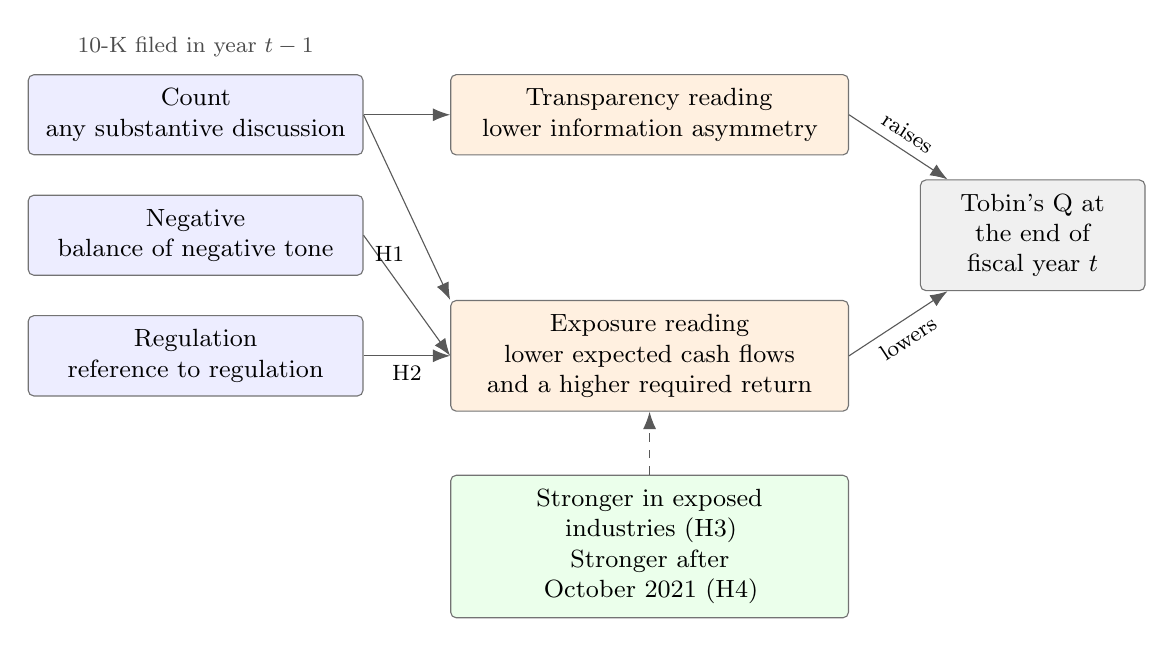
\begin{tikzpicture}[node distance=5mm and 11mm, every node/.style={font=\small},
  box/.style={draw=black!55, rounded corners=2pt, align=center, inner sep=5pt, execute at begin node={\hyphenpenalty=10000\exhyphenpenalty=10000}},
  score/.style={box, fill=blue!7, text width=3.9cm},
  channel/.style={box, fill=orange!12, text width=4.7cm},
  outcome/.style={box, fill=black!6, text width=2.5cm},
  moderator/.style={box, fill=green!8, text width=4.7cm},
  flow/.style={-{Latex[length=2.2mm]}, draw=black!65}]
\node[score] (count) {Count\\ any substantive discussion};
\node[score, below=of count] (neg) {Negative\\ balance of negative tone};
\node[score, below=of neg] (reg) {Regulation\\ reference to regulation};
\node[channel, right=of count] (trans) {Transparency reading\\ lower information asymmetry};
\node[channel, right=of reg] (expo) {Exposure reading\\ lower expected cash flows and a higher required return};
\node[outcome, right=9mm of $(trans.east)!0.5!(expo.east)$] (q) {Tobin's Q at the end of fiscal year $t$};
\node[moderator, below=8mm of expo] (mods) {Stronger in exposed industries (H3)\\ Stronger after October 2021 (H4)};
\node[above=1mm of count, font=\footnotesize, text=black!70] {10-K filed in year $t-1$};
\draw[flow] (count) -- (trans);
\draw[flow] (count.east) -- (expo.north west);
\draw[flow] (neg.east) -- node[pos=0.3, above, font=\footnotesize] {H1} (expo.west);
\draw[flow] (reg) -- node[below, font=\footnotesize] {H2} (expo);
\draw[flow] (trans.east) -- node[above, sloped, font=\footnotesize] {raises} (q);
\draw[flow] (expo.east) -- node[below, sloped, font=\footnotesize] {lowers} (q);
\draw[flow, dashed] (mods) -- (expo);
\end{tikzpicture}
\caption{Conceptual framework and hypotheses}\label{fig:framework}
\tablenote{Note. The Count score can work through both readings, so no sign is predicted for it. The dashed arrow marks the two conditions under which the exposure reading is expected to be stronger.}
\end{figure}

\section{Methodology and data}

\subsection{Data sources}

The study combines two sources. The biodiversity scores come from the public data files that accompany \citet{giglio2026}, obtained from the data page of the authors on 18 November 2026. The firm-level file holds 60,422 rows for 7,236 tickers and the years 2000 to 2024. Each row carries a ticker, a year, a CUSIP and the three scores. Three small files give exposure scores for GICS industry groups, based on the survey of the authors, on the holdings of biodiversity funds and on CDP responses. Accounting and market data come from the Compustat North America Fundamentals Annual file, obtained through WRDS, and the extract covers fiscal years 2013 to 2025 in full. The extra years at both ends are needed for growth rates and for the timing test in Section 3.3. Each raw file is identified by its SHA-256 hash, which is recorded in the data log and checked every time the code runs. Figure~\ref{fig:design} shows the path from the raw files to the tables.

\begin{figure}[!htbp]
\centering
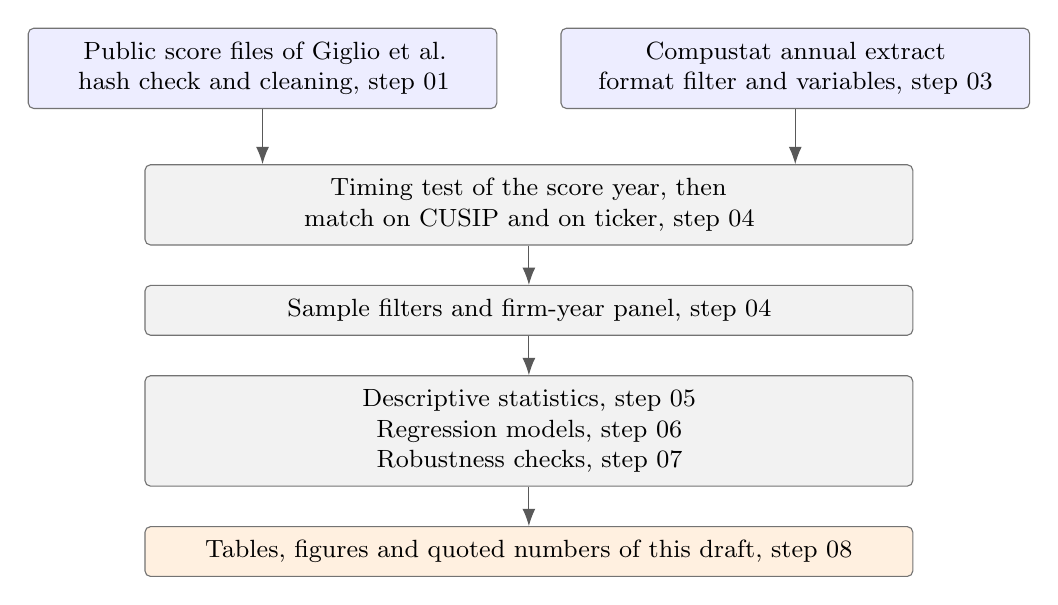
\begin{tikzpicture}[node distance=5mm and 8mm, every node/.style={font=\small},
  box/.style={draw=black!55, rounded corners=2pt, align=center, inner sep=5pt, execute at begin node={\hyphenpenalty=10000\exhyphenpenalty=10000}},
  source/.style={box, fill=blue!7, text width=5.6cm},
  process/.style={box, fill=black!5, text width=9.4cm},
  result/.style={box, fill=orange!12, text width=9.4cm},
  flow/.style={-{Latex[length=2.2mm]}, draw=black!65}]
\node[source] (scores) {Public score files of Giglio et al.\\ hash check and cleaning, step 01};
\node[source, right=of scores] (compustat) {Compustat annual extract\\ format filter and variables, step 03};
\node[process, below=7mm of $(scores.south)!0.5!(compustat.south)$] (timing) {Timing test of the score year, then match on CUSIP and on ticker, step 04};
\node[process, below=of timing] (panel) {Sample filters and firm-year panel, step 04};
\node[process, below=of panel] (models) {Descriptive statistics, step 05\\ Regression models, step 06\\ Robustness checks, step 07};
\node[result, below=of models] (draft) {Tables, figures and quoted numbers of this draft, step 08};
\draw[flow] (scores.south) -- (scores.south |- timing.north);
\draw[flow] (compustat.south) -- (compustat.south |- timing.north);
\draw[flow] (timing) -- (panel);
\draw[flow] (panel) -- (models);
\draw[flow] (models) -- (draft);
\end{tikzpicture}
\caption{Research design from the raw files to the tables}\label{fig:design}
\tablenote{Note. The step numbers refer to the scripts that accompany the paper. Each step checks its inputs before it writes any output.}
\end{figure}

\subsection{Biodiversity scores}

\citet{giglio2026} classify the sentences of each 10-K filing and build three scores. According to the codebook, Count equals one if the filing contains at least two sentences about biodiversity. Negative is the number of biodiversity sentences with a negative tone minus the number with a positive tone. Regulation equals one if the filing contains at least two biodiversity sentences of which at least one concerns regulation. The authors report a precision of 83.6 per cent and a recall of 78.6 per cent in the validation of their classification.

Four features of the file shape the cleaning rules.

\begin{itemize}
\item A total of 458 rows have no CUSIP and no Count or Regulation score. They belong to 76 tickers in the years 2000 to 2018 and are dropped.
\item The year 2000 contains no positive score in any of its 2,743 rows. It is dropped, and the series starts in 2001. Of the 458 rows without a score, 48 lie in the year 2000, so the two rules together remove 3,153 rows.
\item Identifiers are read as text. The file contains the tickers NA and TRUE, and in 7,980 rows the CUSIP begins with a zero. A default import would turn the first into missing values and strip the zeros from the second.
\item In 340 rows Count is zero while Negative is not zero. A single sentence can carry tone without reaching the threshold of two sentences, so Negative is kept as a variable in its own right and is not set to zero when Count is zero.
\end{itemize}

After cleaning, the file holds 57,269 firm-years for 2001 to 2024, with one row per ticker and year. Negative ranges from $-9$ to 8, and Regulation never equals one when Count is zero. The scores for 2024 differ from earlier years in coverage. The file holds 3,728 firms in 2024 against 2,337 in 2023, and 1,176 of the 2024 tickers appear in no earlier year. The main analysis therefore uses scores up to 2023. Because the scores are lagged by one year, Tobin's Q can still be measured up to fiscal year 2024.

\subsection{Timing of the score year}

The codebook does not say whether the year in the file is the fiscal year that a 10-K reports on or the calendar year in which it was filed. For a firm with a December year end the two differ by one, and the wrong reading would shift every regressor by a year. The question was examined in two ways.

The first uses counts in the score file for firms with a December year end (Table~\ref{tab:alignment} in the appendix). Among the \nTrailRows{} rows that lie one year after the last fiscal year with a share price, \nTrailFilled{} carry any score, against \nTrailBeforeFilled{} of \nTrailBefore{} one year earlier. This fits the fiscal year reading if an empty row means that no report exists for that year. Among the rows in the first such fiscal year, \nFirstFilled{} of \nFirstRows{} carry a score, against \nFirstNextFilled{} of \nFirstNext{} one year later. This fits the filing year reading, since many newly listed firms file their first 10-K only in the year after listing. The counts do not decide the question.

The second is a check against filings on EDGAR, made on 23 November 2026. First, an empty last row does not mean that no report was filed. Table~\ref{tab:edgarleavers} lists \nEdgarLeavers{} firms that left the file between 2018 and 2021 with a positive Count score in their second-last year. Each filed a Form 10-K in February or March of its last year, and that row is still empty. Second, for firms that stay, the text changes in the 10-K filed in the score year. For \nEdgarSwitch{} firms whose Count score turns from zero to one, sentences with a biodiversity word were counted in the 10-K filed in the year before, in the year of and in the year after the first positive score. The count rises clearly for \nEdgarClear{} firms. For \nEdgarFiling{} of them the rise is already in the 10-K filed in the score year, and for \nEdgarFiscal{} it comes one filing later (Table~\ref{tab:edgarswitch}). Third, where the text changes sharply the match is exact. Rayonier Advanced Materials has about thirty such sentences in each 10-K filed from 2018 to 2021 and fewer than ten in other years, and its Count score is one in exactly those four years (Table~\ref{tab:edgarhistory}).

The year in the score file is therefore read as the calendar year of filing. This agrees with the remark of \citet{giglio2026} that their portfolios use the filing of the prior year to avoid look-ahead bias. The reading rests on a count of words for large firms that are still listed, and a confirmation by the authors of the scores would settle the matter.

The regressor for Tobin's Q at the end of fiscal year $t$, the score of year $t-1$, thus comes from the 10-K filed in the previous calendar year. Investors could read it before the valuation date whatever the month of the fiscal year end. For a firm with a December year end it was filed about 21 months before that date. The score of year $t$ is the most recent report for such a firm, filed about nine months before the valuation date. It is used in checks R10, W10 and P8, so that each main result can be read under both timings.

\subsection{Sample construction}

The sample starts from all Compustat firm-years with fiscal years 2015 to 2024 in the standard industrial format with consolidated data. Filters are applied in a fixed order, and Figure~\ref{fig:sample} records the number of firm-years and firms left after each step. The firm has to be incorporated in the United States and report in US dollars. Financial firms with SIC codes 6000 to 6999 are excluded. Total assets and the market value of equity have to be positive, and book equity and a GICS industry group have to be available. The firm-year has to be matched to a biodiversity score of the previous year, and all control variables have to be available.

\begin{figure}[!htbp]
\centering
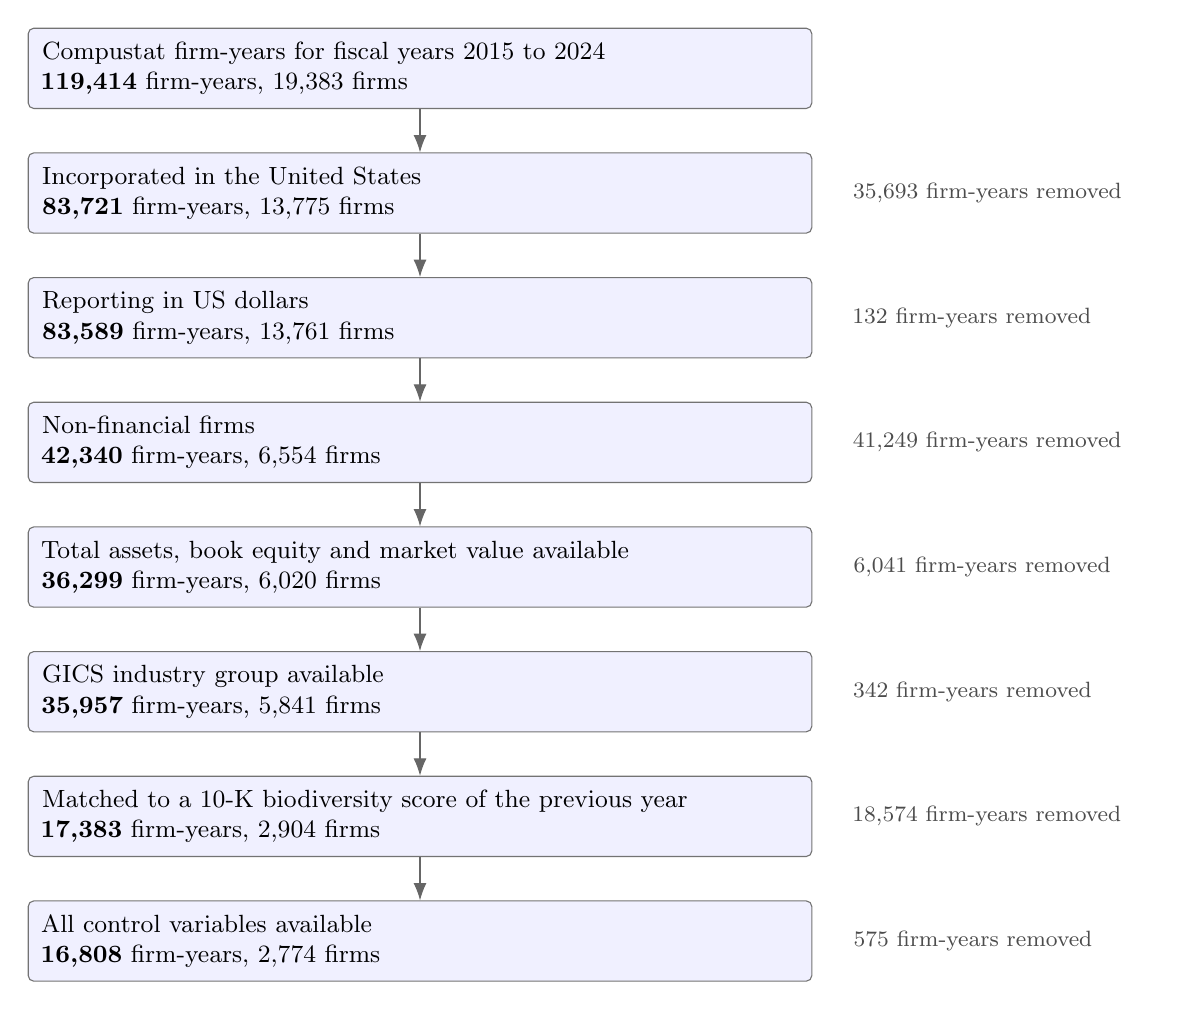
\begin{tikzpicture}[node distance=5.5mm, every node/.style={font=\small},
  stage/.style={draw=black!55, fill=blue!6, rounded corners=2pt, text width=9.6cm, align=left, inner sep=5pt, execute at begin node={\hyphenpenalty=10000\exhyphenpenalty=10000}},
  removed/.style={text width=3.9cm, align=left, text=black!70, font=\footnotesize},
  flow/.style={-{Latex[length=2.2mm]}, draw=black!60}]
\node[stage] (s0)  {Compustat firm-years for fiscal years 2015 to 2024\\ \textbf{119,414} firm-years, 19,383 firms};
\node[stage] (s1) [below=of s0] {Incorporated in the United States\\ \textbf{83,721} firm-years, 13,775 firms};
\draw[flow] (s0) -- (s1);
\node[removed, right=4mm of s1] {35,693 firm-years removed};
\node[stage] (s2) [below=of s1] {Reporting in US dollars\\ \textbf{83,589} firm-years, 13,761 firms};
\draw[flow] (s1) -- (s2);
\node[removed, right=4mm of s2] {132 firm-years removed};
\node[stage] (s3) [below=of s2] {Non-financial firms\\ \textbf{42,340} firm-years, 6,554 firms};
\draw[flow] (s2) -- (s3);
\node[removed, right=4mm of s3] {41,249 firm-years removed};
\node[stage] (s4) [below=of s3] {Total assets, book equity and market value available\\ \textbf{36,299} firm-years, 6,020 firms};
\draw[flow] (s3) -- (s4);
\node[removed, right=4mm of s4] {6,041 firm-years removed};
\node[stage] (s5) [below=of s4] {GICS industry group available\\ \textbf{35,957} firm-years, 5,841 firms};
\draw[flow] (s4) -- (s5);
\node[removed, right=4mm of s5] {342 firm-years removed};
\node[stage] (s6) [below=of s5] {Matched to a 10-K biodiversity score of the previous year\\ \textbf{17,383} firm-years, 2,904 firms};
\draw[flow] (s5) -- (s6);
\node[removed, right=4mm of s6] {18,574 firm-years removed};
\node[stage] (s7) [below=of s6] {All control variables available\\ \textbf{16,808} firm-years, 2,774 firms};
\draw[flow] (s6) -- (s7);
\node[removed, right=4mm of s7] {575 firm-years removed};
\end{tikzpicture}

\caption{Construction of the sample}\label{fig:sample}
\tablenote{Note. Each box applies one more filter to the firm-years that passed the box above it. The counts are written by the code that builds the sample.}
\end{figure}

Scores are matched to Compustat on the first eight characters of the CUSIP and the score year. Firm-years that remain unmatched are then matched on ticker and score year, and a score row is never used twice. Compustat reports the most recent CUSIP of a firm, so firms that changed their CUSIP can be missed in the first step, and the ticker step recovers only part of them. Of the \nGics{} firm-years that pass the earlier filters, \nMatched{} are matched to a score, which is \pctMatched{} per cent. The score file therefore covers about half of the non-financial firm-years in Compustat, and the results describe the firms that it covers. About \pctCusip{} per cent of the firm-years in the final sample are matched on CUSIP. The final sample has \nFinal{} firm-years of \nFirmsFinal{} firms.

\subsection{Variables}

The dependent variable is Tobin's Q at the end of fiscal year $t$,
\begin{equation}
Q_{i,t} = \frac{\mathit{AT}_{i,t} - \mathit{CEQ}_{i,t} + \mathit{PRCC\_F}_{i,t} \times \mathit{CSHO}_{i,t}}{\mathit{AT}_{i,t}},
\end{equation}
where $\mathit{AT}$ is total assets, $\mathit{CEQ}$ is common equity, $\mathit{PRCC\_F}$ is the share price at the fiscal year end and $\mathit{CSHO}$ is the number of shares outstanding. The book value of assets stands in for their replacement cost, which is the usual simplification in this literature.

The control variables are firm size, leverage, profitability, asset tangibility, sales growth, research and development intensity, capital expenditure, cash holdings and an indicator for dividend payers. Missing research and development expense is set to zero and flagged with a separate indicator. All controls are measured in the same fiscal year as Tobin's Q. Tobin's Q and the continuous controls are winsorised at the 1st and 99th percentiles of the pooled sample. Table~\ref{tab:variables} in the appendix gives the definitions and the Compustat items.

Two indicators are used in the further tests. High equals one for firms in industry groups whose survey-based exposure lies above the two-thirds quantile of the non-financial industry groups. Post equals one for fiscal years from 2022, the first fiscal years in which every year end falls after the Kunming Declaration.

\subsection{Empirical models}

The baseline model compares firms within the same industry group and fiscal year,
\begin{equation}
Q_{i,t} = \beta_1 \mathit{Count}_{i,t-1} + \beta_2 \mathit{Negative}_{i,t-1} + \beta_3 \mathit{Regulation}_{i,t-1} + \gamma' X_{i,t} + \mu_{j,t} + \varepsilon_{i,t},
\label{eq:baseline}
\end{equation}
where $i$ is the firm, $t$ the fiscal year and $j$ the GICS industry group. $X$ is the vector of controls, and $\mu_{j,t}$ is a fixed effect for each industry group in each year, which removes differences between industries and shocks common to an industry in a year. H1 predicts a negative $\beta_2$ and H2 a negative $\beta_3$. The second model replaces the industry-by-year effects with firm effects $\alpha_i$ and year effects $\lambda_t$, so that the coefficients are identified from changes within a firm,
\begin{equation}
Q_{i,t} = \beta_1 \mathit{Count}_{i,t-1} + \beta_2 \mathit{Negative}_{i,t-1} + \beta_3 \mathit{Regulation}_{i,t-1} + \gamma' X_{i,t} + \alpha_i + \lambda_t + \varepsilon_{i,t}.
\label{eq:firm}
\end{equation}
Each equation is estimated with the controls only, then with one score at a time, and then with the three scores together. Each table opens with one further column, which enters the three scores with the fixed effects alone and leaves out the controls. It is estimated on the same firm-years as the full model, so the two columns differ only in the controls. It shows how far the fixed effects by themselves account for the raw difference in valuation, and whether the estimates depend on the choice of controls. Some controls, such as profitability and investment, may themselves respond to biodiversity risk, and a model that holds them constant could then understate the association.

H3 and H4 are tested with interaction terms, one score $S$ at a time,
\begin{align}
Q_{i,t} &= \beta S_{i,t-1} + \delta \left( S_{i,t-1} \times \mathit{High}_{j} \right) + \gamma' X_{i,t} + \mu_{j,t} + \varepsilon_{i,t}, \label{eq:high}\\
Q_{i,t} &= \beta S_{i,t-1} + \theta \left( S_{i,t-1} \times \mathit{Post}_{t} \right) + \gamma' X_{i,t} + \mu_{j,t} + \varepsilon_{i,t}. \label{eq:post}
\end{align}
The indicators High and Post do not enter on their own because the fixed effects absorb them. H3 predicts a negative $\delta$ and H4 a negative $\theta$ for the Negative and Regulation scores. Equation~\eqref{eq:post} is also estimated with firm and year fixed effects. Fiscal year 2021 needs care in this test. It covers year ends from June 2021 to May 2022, so a firm with a December year end is valued some weeks after the declaration although the year counts as the earlier period. Equation~\eqref{eq:post} is therefore estimated a third time without fiscal year 2021. For each version the sum of $\beta$ and $\theta$ is also reported with its own standard error. It is the slope of the score from fiscal year 2022.

All models are estimated by ordinary least squares with high-dimensional fixed effects. Standard errors are clustered by firm, because both valuation and disclosure are persistent within firms \citep{petersen2009}. Tests are two-sided, and the 5 per cent level is used as the threshold for a finding. The list of models and the rules for reading them were fixed before any firm-level data were merged. H1 and H2 are read on the model with the three scores together under industry-by-year effects, and the coefficient has to be of the same sign within firms. A result that is significant at the 10 per cent level only, or in one specification only, is weak evidence. Two additions were made after the first timing test and before any regression was run, namely the estimate without fiscal year 2021 and robustness check R10. Three were made after the first results were known, namely the column without controls, the slope from fiscal year 2022 and the further checks of Section 3.8. These are reported for information and have no part in the rules by which the hypotheses are read.

\subsection{Identification and its limits}

The estimates are associations, and four features of the setting limit a causal reading. These are the standard sources of endogeneity in corporate finance \citep{roberts2013}.

The first is that disclosure is a choice. Managers decide what to write, so a coefficient on a score mixes the effect of the underlying exposure with the effect of disclosing it. Entering the three scores separately reduces this problem but does not remove it. The second is omitted variables. The business model or location of a firm may drive both what it discloses and how it is valued. Industry-by-year effects remove differences between industries, and firm effects remove firm traits that do not change over time. Traits that change over time remain a concern. The third is reverse causality. A fall in valuation could itself lead managers to write more about risk. Lagging the scores by one year rules out an effect of the valuation of the same year on the text, although persistent shocks can still run in that direction.

The fourth is specific to these scores. A positive score is rare and persistent, so estimates with firm fixed effects rest on the few firms whose score changes. The model with industry-by-year effects is therefore the main specification, and the model with firm effects is reported beside it. A placebo test adds a further check across firms. If investors respond to what a firm discloses, the score that the firm will report two years later should not explain the valuation of today once the current scores are in the model. If it does, a lasting firm trait is at work. Firm effects already remove such traits, so for the within-firm estimates the concern is a shock that changes over time. Two of the checks in Section 3.8 address it.

\subsection{Robustness checks}

Ten checks re-estimate the model for one score at a time with the full set of controls.

\begin{itemize}
\item R1 uses the natural logarithm of Tobin's Q.
\item R2 uses Tobin's Q minus the median of its industry group and year, with year fixed effects.
\item R3 excludes utilities, whose prices are regulated.
\item R4 excludes fiscal year 2020, the first year of the pandemic.
\item R5 keeps only firms with a December year end, for which fiscal and calendar years coincide.
\item R6 keeps only firm-years matched on CUSIP.
\item R7 keeps only firms that have a positive Count score at least once, with firm and year fixed effects.
\item R8 clusters standard errors by industry group. With about twenty clusters these standard errors are indicative only.
\item R9 is the placebo test with the score that the firm reports two years later.
\item R10 uses the score of the same year in place of the score of the previous year. For a firm with a December year end this is the most recent filing before the valuation date.
\end{itemize}

These ten checks are aimed at the comparison across firms. Two results of the paper come from other models, so the main checks were repeated on them after the first results were known. Checks W0 to W10 concern the coefficient on Negative with firm and year effects, with the three scores together and alone. W1 and W3 to W8 follow R1 and R3 to R8. W2 adds industry-by-year effects to the firm effects, W9 adds the Negative score of two years later, and W10 uses the score of the same year. Checks P0 to P9 concern the interaction of Regulation with Post. P1 to P7 follow R1 to R6 and R8, P8 uses the score of the same year, and P9 enters the three scores and their interactions together.

\subsection{Reproducibility}

The analysis is run by numbered scripts from the raw files to the tables. Each step checks its inputs before it writes anything. The checks cover the hashes of the raw files, the uniqueness of firm-years after every merge and the number of observations lost at each filter. A test suite runs the whole pipeline on a synthetic data set with a known coefficient and compares the fixed-effects estimator with a dummy-variable regression. The synthetic data are used for testing only. The tables in this draft and the numbers quoted in the text are written by the last script from the same unrounded estimates, so a number in the text cannot differ from the same number in a table.

\section{Empirical results and discussion}

\subsection{Disclosure scores over time}

Figure~\ref{fig:share} shows, for each year, the share of firms in the score file with a positive Count score and with a positive Regulation score. Discussion of biodiversity in 10-K filings was rare at the start of the period and has grown more than fourfold. The rise is not smooth. The share fell between 2017 and 2021 and rose again in 2022. Part of the fall comes from the denominator, since the number of firms in the file grew from 2,285 in 2019 to 2,843 in 2021 while the number of firms with a positive score stayed between 93 and 105. Score year 2022 refers to annual reports filed in 2022, after the Kunming Declaration of October 2021 and mostly before the Kunming-Montreal framework was adopted in December 2022.

\begin{figure}[!htbp]
\centering
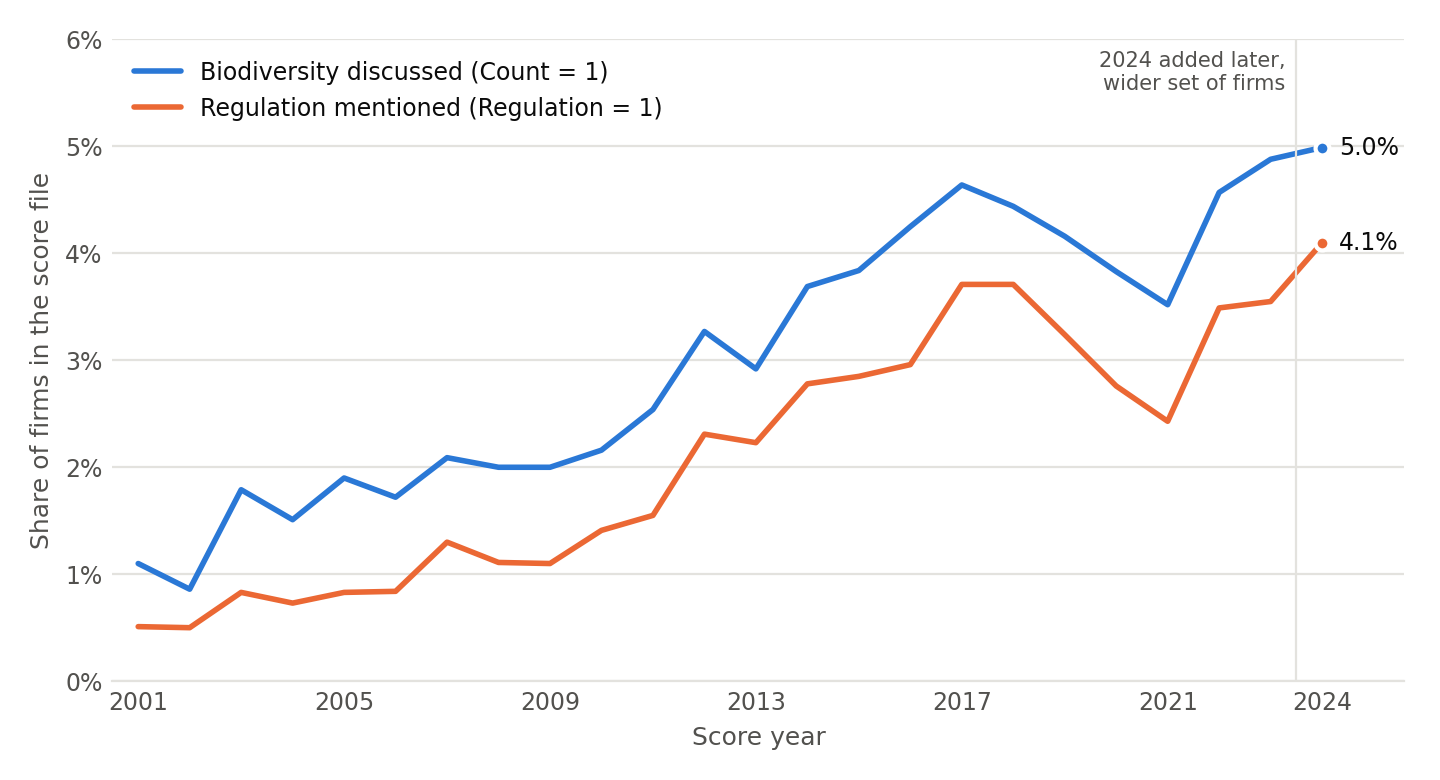
\includegraphics[width=0.92\linewidth]{figures/BRFV_F01_disclosure_share_by_year.png}
\caption{Share of firms with a positive biodiversity score in their 10-K filing, 2001 to 2024}\label{fig:share}
\tablenote{Source. Score file of \citet{giglio2026}, 57,269 firm-years. Calculations of the author.}
\end{figure}

Table~\ref{tab:period} groups the years into periods and adds the tone of the discussion. Regulation accounts for a growing part of the discussion. Half of the firm-years with a positive Count score also had a positive Regulation score in 2001 to 2007, against three quarters in 2015 to 2023. The shares for 2015 to 2023 agree with those that \citet{giglio2026} report for the same years, which are about 4.2 per cent for biodiversity and 3.2 per cent for regulation. This confirms that the file has been read correctly. The tone is negative far more often than positive. In 2015 to 2023 the Negative score is above zero in 494 firm-years and below zero in 131.

\begin{table}[!htbp]
\centering\small
\caption{Biodiversity scores in 10-K filings by period}\label{tab:period}
\widetable{tables/tab_scores_by_period}
\tablenote{Source. Score file of \citet{giglio2026}. Firm-years are rows with valid scores. The last two columns count all firm-years, including those with a Count score of zero.}
\end{table}

\subsection{Persistence of disclosure}

Table~\ref{tab:persistence} follows firms from one year to the next. Few firms ever have a positive score. In 2015 to 2023 this holds for 263 of 3,746 firms, or 7 per cent. The score is also sticky. A firm with a positive score keeps it in the next year in 80 per cent of cases, while a firm without one acquires it in less than 1 per cent of cases. As a result only 215 firms change status in 2015 to 2023.

\begin{table}[!htbp]
\centering\small
\caption{Persistence of the Count score}\label{tab:persistence}
\widetable{tables/tab_persistence}
\tablenote{Source. Score file of \citet{giglio2026}. Firms are identified by ticker. The last two columns are computed over pairs of consecutive years for the same firm.}
\end{table}

\subsection{Industry exposure and industry disclosure}

Table~\ref{tab:industry} lists the survey-based exposure scores of \citet{giglio2026} for the GICS industry groups, together with the place of each group in the regression sample. A higher survey value means that respondents rate the industry as more exposed. Seven of the twenty non-financial industry groups lie above the two-thirds quantile and form the high-exposure group.

The right-hand columns show that disclosure follows a different pattern. A positive Count score is found in \pctEnergy{} per cent of the firm-years in Energy, in \pctUtilities{} per cent in Utilities and in \pctMaterials{} per cent in Materials. These three groups hold \pctTopThree{} per cent of all firm-years with a positive score. In Food, Beverage and Tobacco and in the two health care groups, which the survey also rates as highly exposed, the share is below 2 per cent, and in Transportation it is \pctTransport{} per cent. The survey therefore captures where respondents see exposure, while the 10-K scores capture where firms write about it. The two agree for energy, utilities and materials and differ for food, health care and transportation, which matters for the test of H3.

\begin{table}[!htbp]
\centering\small
\caption{Survey-based exposure and disclosure by GICS industry group}\label{tab:industry}
\widetable{tables/tab_industry}
\tablenote{Source. Survey file of \citet{giglio2026} and the regression sample. Average is the mean of the transition and physical scores. High marks groups above the two-thirds quantile of the non-financial groups. Firms are screened on SIC codes, so a few firms with a financial GICS code remain in the sample. Real Estate and Insurance lie above the cut-off, so their \nHighFinFY{} firm-years count as high exposure in the regressions. One group has no survey score.}
\end{table}

\subsection{Sample and descriptive statistics}

Table~\ref{tab:summary} reports summary statistics for the \nFinal{} firm-years of the sample. The mean of Tobin's Q is \meanQ{} and the median is \medianQ{}. A positive Count score is found in \pctCount{} per cent of the firm-years and a positive Regulation score in \pctReg{} per cent. About \pctHigh{} per cent of the firm-years belong to high-exposure industries, and about \pctDecember{} per cent have a December year end.

\begin{table}[!htbp]
\centering\small
\caption{Summary statistics}\label{tab:summary}
\widetable{tables/tab_summary}
\tablenote{Note. The three scores are those of the previous year. Tobin's Q and the continuous controls are winsorised at the 1st and 99th percentiles. Table~\ref{tab:variables} gives the definitions.}
\end{table}

Table~\ref{tab:means} compares firm-years with and without a positive Count score, and Figure~\ref{fig:qgroups} shows the mean of Tobin's Q for the two groups in each fiscal year. Firms that discuss biodiversity are valued much lower. Their mean Tobin's Q is \meanQOne{}, against \meanQZero{} for the other firm-years, and the gap is present in every year. The same firms are larger, hold far more tangible assets, with a tangibility of \tangOne{} against \tangZero{}, invest more, spend little on research and development and hold less cash. These are the features of asset-heavy industries, which are valued lower for reasons that have nothing to do with disclosure. The raw gap therefore cannot be read as an effect of biodiversity disclosure.

\begin{table}[!htbp]
\centering\small
\caption{Firm-years with and without a positive Count score}\label{tab:means}
\widetable{tables/tab_means}
\tablenote{Note. The last column is a Welch $t$ statistic. Firm-years are not independent, so it is a description and not a test.}
\end{table}

\begin{figure}[!htbp]
\centering
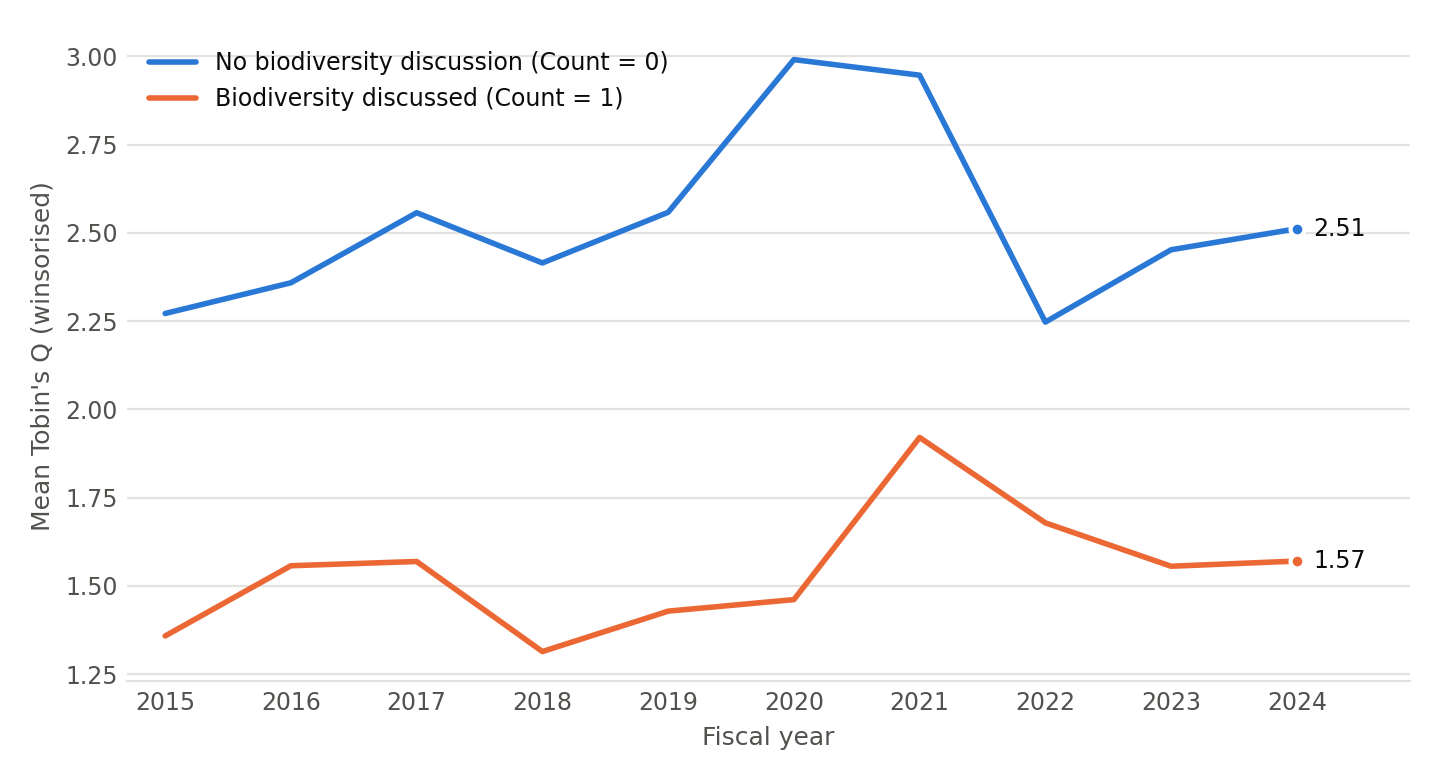
\includegraphics[width=0.88\linewidth]{figures/BRFV_F02_tobin_q_by_disclosure.png}
\caption{Mean Tobin's Q by disclosure status and fiscal year}\label{fig:qgroups}
\tablenote{Source. Regression sample, \nFinal{} firm-years. Tobin's Q is winsorised.}
\end{figure}

Table~\ref{tab:variation} shows how much variation the scores offer. Only \nEverCount{} firms have a positive Count score in at least one year, and \nChangeCount{} of them change status within the sample. The Negative score changes over time for \nChangeNeg{} firms and the Regulation score for \nChangeReg{} firms. Estimates with firm fixed effects rest on these firms.

\begin{table}[!htbp]
\centering\small
\caption{Variation in the scores within the sample}\label{tab:variation}
\widetable{tables/tab_variation}
\tablenote{Note. A firm contributes to an estimate with firm fixed effects only if its score changes over time.}
\end{table}

\subsection{Biodiversity scores and Tobin's Q}

Table~\ref{tab:baseline} reports equation~\eqref{eq:baseline}. Column 1 enters the three scores with the industry-by-year effects alone. The coefficient on Count is \coefBNoCount{} with a standard error of \seBNoCount{}. It is small beside the raw difference of \gapQ{} in Section 4.4 and is not significant, and the coefficients on Negative and Regulation are close to zero. The remaining columns add the controls. With industry-by-year effects and controls, none of the three scores is related to Tobin's Q. The coefficient on Count is \coefBCount{} with a standard error of \seBCount{} when it enters alone. The coefficients on Negative and Regulation are \coefBNeg{} and \coefBReg{}, and both are well within one standard error of zero. When the three scores enter together in column 6, the coefficient on Count is \coefBAllCount{}, the coefficient on Negative is \coefBAllNeg{} and the coefficient on Regulation is \coefBAllReg{}, and none is significant. The controls raise the $R^2$ from \rsqBNo{} to \rsqB{} and do not change the conclusion. The large raw gap of Section 4.4 is thus explained first by industry and year, and the small remainder by firm characteristics.

\begin{table}[!htbp]
\centering\small
\caption{Biodiversity scores and Tobin's Q with industry-by-year effects}\label{tab:baseline}
\widetable{tables/tab_baseline}
\tablenote{Note. The dependent variable is Tobin's Q. Scores are those of the previous year. Column 1 leaves out the controls and is estimated on the firm-years of column 6. Firms are counted on the firm-years that enter the estimate. Standard errors clustered by firm are in parentheses. One, two and three stars mark significance at the 10, 5 and 1 per cent levels. The model labels are those used in the code.}
\end{table}

Table~\ref{tab:firm} reports equation~\eqref{eq:firm}. The \nFirmsOnce{} firms with a single firm-year drop out, so the estimates rest on \nObsF{} firm-years of \nFirmsF{} firms. Within firms, the Count and Regulation scores remain unrelated to valuation, with or without the controls. The Negative score behaves differently, and the result depends on the column. Alone, its coefficient is \coefFNeg{} with a $p$ value of \pvalFNeg{}, which misses the 5 per cent threshold. With the three scores together it is \coefFAllNeg{}, with a standard error of \seFAllNeg{} and a $p$ value of \pvalFAllNeg{}. The rule fixed in advance refers to the second of these columns. The two differ because the scores are correlated. Count and Regulation have a correlation of \corrCountReg{} in the sample (Table~\ref{tab:correlations} in the appendix) and \corrInCountReg{} within firms, so their separate coefficients in column 6 are imprecise and should not be read one by one. Negative is less correlated with the other two, at \corrInCountNeg{} and \corrInNegReg{} within firms, and its standard error is almost the same in both columns. What moves is the point estimate, because Negative alone also reflects the two scores that are left out. Without the controls, in column 1, the coefficient is nearly twice as large. The controls thus take away about half of the association. They may remove a part that is not due to biodiversity, or they may lie on the path from biodiversity risk to value. The estimate with controls remains the main one, as was fixed in advance. One more negative sentence goes with a Tobin's Q that is lower by about \effNegMean{} per cent of the sample mean, or \effNegDisc{} per cent of the mean of the firm-years with a positive Count score. Figure~\ref{fig:coefficients} sets the two sets of estimates side by side.

\begin{table}[!htbp]
\centering\small
\caption{Biodiversity scores and Tobin's Q with firm and year effects}\label{tab:firm}
\widetable{tables/tab_firm_effects}
\tablenote{Note. The dependent variable is Tobin's Q. Scores are those of the previous year. Firms with one firm-year drop out and are not counted. Column 1 leaves out the controls and is estimated on the firm-years of column 6. Standard errors clustered by firm are in parentheses. One, two and three stars mark significance at the 10, 5 and 1 per cent levels.}
\end{table}

\begin{figure}[!htbp]
\centering
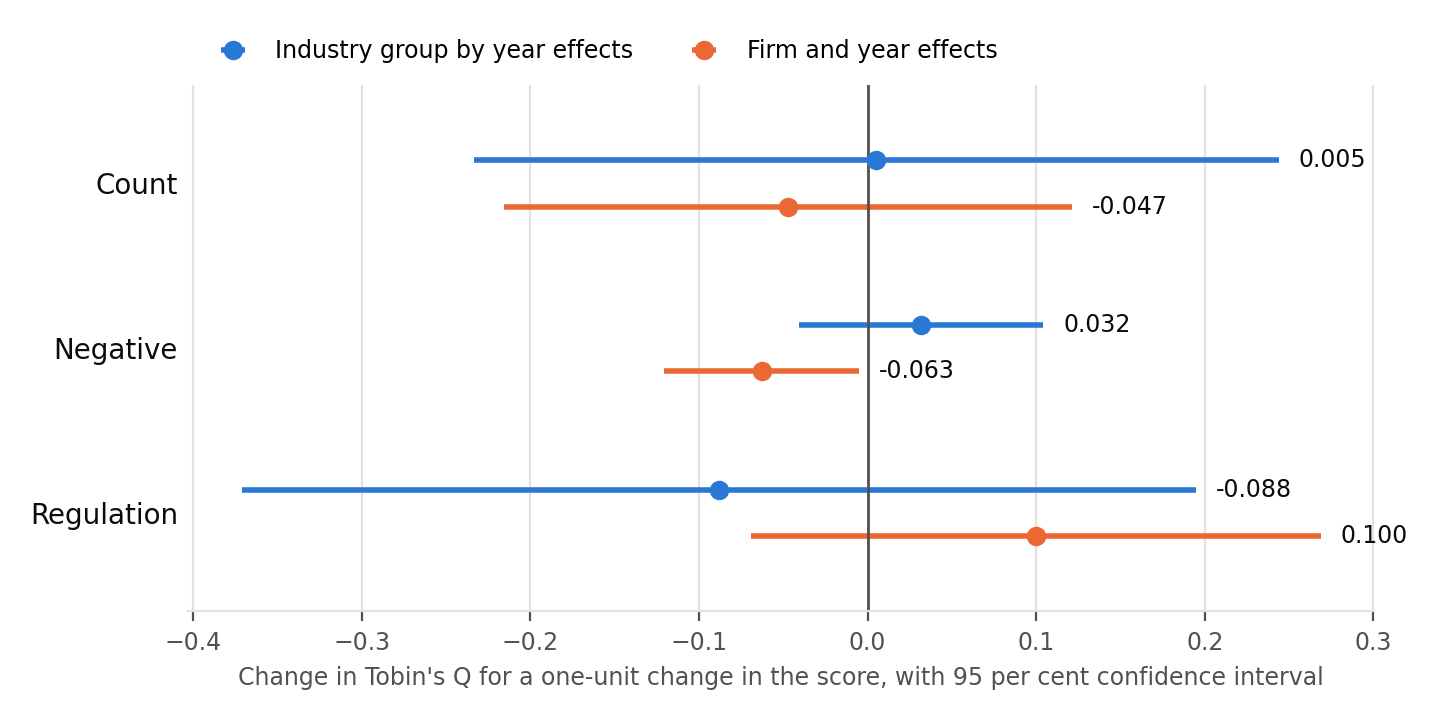
\includegraphics[width=0.9\linewidth]{figures/BRFV_F03_coefficients_main.png}
\caption{Coefficients on the three scores under the two specifications}\label{fig:coefficients}
\tablenote{Source. Column 6 of Table~\ref{tab:baseline} and column 6 of Table~\ref{tab:firm}. The lines show 95 per cent confidence intervals.}
\end{figure}

The rule for reading these tables was fixed in advance. H1 would be supported if the coefficient on Negative in the model with the three scores together were negative and significant at the 5 per cent level under industry-by-year effects, and of the same sign within firms. Column 6 of Table~\ref{tab:baseline} shows no association, so H1 is not supported. The within-firm estimate is negative and significant in one specification only. By the same rules it is weak evidence, confined to changes within firms. H2 is not supported. The coefficient on Regulation is not significant in either specification and changes sign between them. The coefficient on Count, for which no sign was predicted, is not significant in any column.

\subsection{Industry exposure and the period after October 2021}

Table~\ref{tab:exposure} reports equation~\eqref{eq:high}. The interaction of each score with the high-exposure indicator is small relative to its standard error. For the Negative score the interaction is \coefXNeg{} with a standard error of \seXNeg{}, and for the Regulation score it is \coefXReg{} with a standard error of \seXReg{}. H3 is not supported. Section 4.3 suggests one reason. The high-exposure group holds the three industries in which most of the discussion takes place, together with food, health care and transportation, where firms hardly discuss biodiversity. Outside the group a positive score is rare, so the slope for the other industries rests on few firm-years and the difference between the two slopes is imprecise.

\begin{table}[!htbp]
\centering\small
\caption{Biodiversity scores and Tobin's Q in high-exposure industries}\label{tab:exposure}
\widetable{tables/tab_exposure}
\tablenote{Note. The dependent variable is Tobin's Q. High marks industry groups above the two-thirds quantile of the survey-based exposure score. The indicator itself is absorbed by the fixed effects. Controls are included. Standard errors clustered by firm are in parentheses.}
\end{table}

Table~\ref{tab:event} reports equation~\eqref{eq:post}. The result differs by score. For the Regulation score the interaction with Post is \coefEReg{} with a standard error of \seEReg{} and a $p$ value of \pvalEReg{} in the main specification. The slope before fiscal year 2022 is \coefPreEReg{}, so a discussion of regulation was then unrelated to valuation. The slope from fiscal year 2022 is \coefSlopeEReg{} with a standard error of \seSlopeEReg{} and a $p$ value of \pvalSlopeEReg{}. The change between the periods is thus significant, while the association in the later period is not itself distinguishable from zero. The estimate without fiscal year 2021 is \coefEDReg{} with a $p$ value of \pvalEDReg{}, so the change does not depend on the transition year. Within firms the interaction is \coefEFReg{} and not significant. For the Negative score the interaction has the predicted sign in all three versions but is not significant, with \coefENeg{} in the main specification and \coefEFNeg{} within firms. Within firms the slope of the Negative score is \coefPreEFNeg{} before fiscal year 2022 and \coefSlopeEFNeg{} from that year, with a $p$ value of \pvalSlopeEFNeg{} for the latter, although the two do not differ significantly. For the Count score there is no change.

\begin{table}[!htbp]
\centering\footnotesize
\caption{Biodiversity scores and Tobin's Q after the Kunming Declaration}\label{tab:event}
\widetable{tables/tab_event}
\tablenote{Note. The dependent variable is Tobin's Q. Post equals one for fiscal years from 2022 and is absorbed by the year effects. Columns 7 to 9 repeat columns 1 to 3 without fiscal year 2021. The last row is the sum of the coefficients on the score and on its interaction, with its own standard error. Controls are included. Standard errors clustered by firm are in parentheses. Two stars mark significance at the 5 per cent level.}
\end{table}

By the rule fixed in advance, H4 is supported for the Regulation score, since the interaction is negative and significant at the 5 per cent level and holds when fiscal year 2021 is left out. The support is partial. It does not extend to the Negative score, and it is not confirmed within firms, where few firms change their Regulation score after 2021. The slope from fiscal year 2022 is not significant, and by the same rules a result in one specification only is weak evidence.

\subsection{Robustness}

Table~\ref{tab:robustness} in the appendix reports the ten checks. The absence of an association in the comparison across firms is stable. It holds in checks R1 to R6 and R8, which change the measure of Tobin's Q, the sample or the clustering. Check R10, which uses the score of the same year, gives the same picture, so this conclusion does not depend on which filing is used. The placebo test in R9 finds no relation between the valuation of today and the scores that a firm reports two years later. The coefficients are \coefRNineCount{} for Count, \coefRNineNeg{} for Negative and \coefRNineReg{} for Regulation, and none is significant. The test is run across firms, where no association was found to begin with, so it says little about the within-firm result.

Table~\ref{tab:tonechecks} reports checks W0 to W10 on the within-firm result for tone. In W1 to W8 the coefficient on Negative from the model with the three scores is negative in all \nNegWJ{} checks and significant at the 5 per cent level in \nSigWJ{}. With Negative alone it is significant in \nSigWA{}. It is largest among the firms that ever have a positive Count score, as in R7. The two exceptions matter. Without utilities the $p$ value is \pvalWThreeJ{}. With industry-by-year effects added to the firm effects, in W2, the coefficient falls to \coefWTwoJ{} with a standard error of \seWTwoJ{}. This check compares each firm with its own industry group in the same year, and the result does not pass it. The within-firm association can therefore not be separated from shocks that reach a whole industry group in a year. In W9 the coefficient on the Negative score of two years later is \coefWNineLeadJ{} with a $p$ value of \pvalWNineLeadJ{}, so there is no sign that valuation falls before the tone changes, although the test has little power. In W10, with the score of the same year, the coefficient is \coefWTenJ{} and not significant. The association appears with the filing of the previous year and not with the most recent one, which is hard to reconcile with a prompt response of investors to the text.

Table~\ref{tab:regchecks} reports checks P0 to P9 on the interaction of Regulation with Post. In P1 to P7 the interaction is negative in all \nNegPIx{} checks and significant at the 5 per cent level in \nSigPIx{}. It is not significant for firms with a December year end, where it is \coefPFiveIx{} with a $p$ value of \pvalPFiveIx{}. The slope from fiscal year 2022 is significant in \nSigPSlope{} of the seven. With the score of the same year, in P8, the interaction is \coefPEightIx{} with a $p$ value of \pvalPEightIx{}, so the change is found under both timings. When the three scores and their interactions enter together, in P9, the interaction for Regulation is \coefPNineIx{} with a standard error of \sePNineIx{} and is significant at the 10 per cent level only. Count and Regulation are too closely correlated for the change after 2021 to be tied to the regulatory content in particular.

Table~\ref{tab:verdict} brings the tests together.

\begin{table}[!htbp]
\centering\small
\caption{Hypotheses and outcomes}\label{tab:verdict}
\begin{tabularx}{\linewidth}{@{}>{\raggedright\arraybackslash}p{4.3cm}>{\raggedright\arraybackslash}p{3.6cm}>{\raggedright\arraybackslash}p{3.3cm}>{\raggedright\arraybackslash}X@{}}
\toprule
Hypothesis & Across firms in an industry and year & Within firms & Outcome \\
\midrule
H1. Higher Negative score, lower Q & \coefBAllNeg{}, not significant & \coefFAllNeg{}, significant at 5 per cent. \coefWTwoJ{} with industry-by-year effects added & Not supported. Weak evidence within firms, not confirmed by the added checks. \\
\addlinespace
H2. Regulation discussed, lower Q & \coefBAllReg{}, not significant & \coefFAllReg{}, not significant & Not supported. \\
\addlinespace
H3. Stronger in exposed industries & Interactions not significant & Not estimated & Not supported. \\
\addlinespace
H4. Stronger after October 2021 & Regulation \coefEReg{}, significant at 5 per cent. Slope from 2022 \coefSlopeEReg{} and Negative \coefENeg{}, not significant & Regulation \coefEFReg{} and Negative \coefEFNeg{}, not significant & Supported for Regulation across firms, as weak evidence. Not confirmed within firms. \\
\addlinespace
Count, no predicted sign & \coefBAllCount{}, not significant & \coefFAllCount{}, not significant & No association. \\
\bottomrule
\end{tabularx}
\tablenote{Note. The entries are the coefficients from Tables~\ref{tab:baseline}, \ref{tab:firm}, \ref{tab:event} and \ref{tab:tonechecks}. For H4 the entries are the interactions with Post unless stated.}
\end{table}

\subsection{Discussion}

\subsubsection{Interpretation of the findings}

The first finding is that the mere mention of biodiversity in a 10-K filing is not priced. Firms that discuss biodiversity are valued far lower than other firms, but they are energy producers, utilities and materials firms with heavy tangible assets, and the gap disappears once firms are compared with their industry peers. The Count score, which was entered as a benchmark without a predicted sign, is close to zero in every specification. Neither the exposure reading nor the transparency reading of disclosure leaves a trace at this level. One possibility is that the two offset each other. Another is that a mention of biodiversity in the risk section tells investors little that they do not already know from the industry of the firm.

The second finding concerns tone, and it is weaker. When the discussion of a firm turns more negative, its valuation is lower afterwards. The estimate comes from the \nChangeNeg{} firms whose Negative score changes within the sample, and its sign is in line with the exposure reading. Several cautions apply. The estimate passes the 5 per cent threshold only when the three scores enter together. It loses two thirds of its size when each firm is compared with its own industry group in the same year, so a bad year for an industry, in which firms write more negatively and are valued lower, may lie behind it. It is absent when the most recent filing is used. A more negative discussion may also follow an adverse event at the firm, such as a regulatory action or a dispute over land, and the fall in value may reflect the event and not the wording.

The third finding concerns regulation. Until fiscal year 2021 a discussion of biodiversity regulation was unrelated to valuation. From fiscal year 2022 the estimated association is negative, and the change between the two periods is significant. This matches the evidence of \citet{garel2024}, who find that investors began to price biodiversity footprints after the Kunming Declaration and who point to the risk of future regulation. The result should still be read with care. The association after 2021 is not significant taken by itself, and the change is not significant for firms with a December year end. It is one significant interaction among three scores, it cannot be told apart from a change for disclosure in general, and it is not confirmed within firms. The paper does not claim that the declaration caused the change.

The fourth finding is that the survey-based measure of industry exposure does not moderate any association. As Section 4.3 shows, the high-exposure group mixes industries in which the scores vary with industries in which they are almost always zero, so the test has little power.

\subsubsection{Relation to earlier studies}

The results help to place the earlier estimates. The positive association between disclosure and Tobin's Q in \citet{he2024} is not confirmed once industry-by-year effects, a lag and separate scores are used. The US sub-sample of \citet{cosma2025} gives a negative coefficient on the Negative score, and the within-firm estimate of this paper agrees with it in sign. Their positive coefficient on the Regulation score is not confirmed, and after 2021 the sign is negative. The finding of \citet{bach2025} that biodiversity risk goes with weaker performance is consistent in sign with the result on tone, weak as that result is. The studies on cash holdings by \citet{ahmad2024} and \citet{wang2026} show that managers respond to biodiversity risk. The present results suggest that investors respond more selectively.

\subsubsection{Limitations}

Several limitations remain. The scores measure what firms write and not their exposure, and they are positive for few firms. The within-firm estimates rest on fewer than two hundred firms and may not describe firms in general. The score file covers about half of the non-financial firm-years in Compustat, and the firms it covers may differ from those it does not. The reading of the score year as the year of filing rests on a check of a limited number of large firms and is not confirmed by the authors of the scores. Under it the main regressor is not the most recent report. The models do not control for firm-level climate change exposure. The measure of \citet{sautner2023} is public and was not merged for this version, although \citet{giglio2026} find biodiversity and climate exposure to be almost unrelated. Tobin's Q uses the book value of assets in place of their replacement cost, and its distribution remains skewed after winsorising, with a maximum of \maxQ{}. Several hypotheses were tested on three scores, which raises the chance that one result is significant by accident, and the checks on the two findings were chosen after the first results were known. The sample covers firms incorporated in the United States, which is not a party to the Convention on Biological Diversity, so the results may not carry over to jurisdictions with mandatory reporting on nature. The estimates are associations and not causal effects.

\section{Conclusions}

This paper set out to test whether the discussion of biodiversity risk in 10-K filings is reflected in the valuation of US firms. The design separates the fact of disclosure from its tone and its regulatory content, lags the scores by one year, and compares estimates across firms within an industry and year with estimates within firms.

The answer has three parts. The fact of disclosure is not related to valuation. Firms that discuss biodiversity are valued lower, but this reflects the industries they belong to. A more negative tone is followed by lower valuation within the same firm, with a coefficient of \coefFAllNeg{} for one more negative sentence. This is weak evidence. It does not hold once each firm is compared with its own industry group in the same year, and it is absent with the most recent filing. A discussion of regulation is associated with lower valuation only from fiscal year 2022, the first fiscal years that end after the Kunming Declaration of October 2021. The change from the earlier years is significant, while the association in the later years is not yet distinguishable from zero. The measure of industry exposure used here does not change these associations.

For those who use the 10-K scores, the paper offers three practical points. A positive score is rare and sticky, so any estimate with firm fixed effects depends on a small group of firms and should report how many. The year in the score file appears to be the calendar year of filing, so a lag of one year reaches back to the report filed in the previous calendar year. The last year of a firm in the file carries no score although a report was filed in that year, so an empty row should not be mistaken for a filing without biodiversity content.

Disclosure standards are changing. The recommendations of the Taskforce on Nature-related Financial Disclosures and the exposure draft of the International Sustainability Standards Board point towards more structured reporting on nature \citep{tnfd2023,issb2026}. Future work can test whether structured disclosure is priced differently from the narrative in 10-K filings, whether measures of impact such as the corporate biodiversity footprint identify the same firms as measures of disclosure, and whether the result on regulation holds as more years become available.

\section*{Data and code availability}
\addcontentsline{toc}{section}{Data and code availability}

The biodiversity scores are public and can be obtained from the data page of \citet{giglio2026} at \url{https://www.biodiversityrisk.org/download/}. Compustat data are licensed and cannot be shared, but the extract can be rebuilt from the query specification that accompanies the code. The code that produces every table, figure and quoted number is available from the author, together with the small file of filing dates and sentence counts taken from EDGAR.

\addcontentsline{toc}{section}{References}
\begin{thebibliography}{99}
\setlength{\itemsep}{2pt}

\bibitem[Ahmad and Karpuz(2024)]{ahmad2024} Ahmad, M.F. and Karpuz, A. (2024) Beyond climate change risk: biodiversity and corporate cash holdings. \emph{Economics Letters}, 236, 111608. \url{https://doi.org/10.1016/j.econlet.2024.111608}

\bibitem[Bach, Hoang and Le(2025)]{bach2025} Bach, T.N., Hoang, K. and Le, T. (2025) Biodiversity risk and firm performance: evidence from US firms. \emph{Business Strategy and the Environment}, 34(1), 1113--1132. \url{https://doi.org/10.1002/bse.4039}

\bibitem[Berkman, Jona and Soderstrom(2024)]{berkman2024} Berkman, H., Jona, J. and Soderstrom, N. (2024) Firm-specific climate risk and market valuation. \emph{Accounting, Organizations and Society}, 112, 101547. \url{https://doi.org/10.1016/j.aos.2024.101547}

\bibitem[Bolton and Kacperczyk(2021)]{bolton2021} Bolton, P. and Kacperczyk, M. (2021) Do investors care about carbon risk? \emph{Journal of Financial Economics}, 142(2), 517--549. \url{https://doi.org/10.1016/j.jfineco.2021.05.008}

\bibitem[Campbell et~al.(2014)]{campbell2014} Campbell, J.L., Chen, H., Dhaliwal, D.S., Lu, H. and Steele, L.B. (2014) The information content of mandatory risk factor disclosures in corporate filings. \emph{Review of Accounting Studies}, 19(1), 396--455. \url{https://doi.org/10.1007/s11142-013-9258-3}

\bibitem[{Convention on Biological Diversity}(2022)]{cbd2022} Convention on Biological Diversity (2022) \emph{Kunming-Montreal Global Biodiversity Framework}. Decision 15/4 of the Conference of the Parties, adopted 19 December 2022 (CBD/COP/DEC/15/4). Montreal: Secretariat of the Convention on Biological Diversity.

\bibitem[Coqueret, Giroux and Zerbib(2025)]{coqueret2025} Coqueret, G., Giroux, T. and Zerbib, O.D. (2025) The biodiversity premium. \emph{Ecological Economics}, 228, 108435. \url{https://doi.org/10.1016/j.ecolecon.2024.108435}

\bibitem[Cosma et~al.(2025)]{cosma2025} Cosma, S., Cosma, S., Pennetta, D. and Rimo, G. (2025) Does biodiversity matter for firm value? \emph{Journal of International Financial Markets, Institutions and Money}, 105, 102240. \url{https://doi.org/10.1016/j.intfin.2025.102240}

\bibitem[Dasgupta(2021)]{dasgupta2021} Dasgupta, P. (2021) \emph{The economics of biodiversity: the Dasgupta Review}. London: HM Treasury.

\bibitem[Flammer, Giroux and Heal(2025)]{flammer2025} Flammer, C., Giroux, T. and Heal, G.M. (2025) Biodiversity finance. \emph{Journal of Financial Economics}, 164, 103987. \url{https://doi.org/10.1016/j.jfineco.2024.103987}

\bibitem[Garel et~al.(2024)]{garel2024} Garel, A., Romec, A., Sautner, Z. and Wagner, A.F. (2024) Do investors care about biodiversity? \emph{Review of Finance}, 28(4), 1151--1186. \url{https://doi.org/10.1093/rof/rfae010}

\bibitem[Giglio et~al.(2026)]{giglio2026} Giglio, S., Kuchler, T., Stroebel, J. and Zeng, X. (2026) Biodiversity risk. \emph{Review of Finance}, 30(1), 131--161. \url{https://doi.org/10.1093/rof/rfaf063}

\bibitem[He(2024)]{he2024} He, X. (2024) An empirical study on biodiversity disclosure and firm's market value in North America based on linear regression model. \emph{Highlights in Business, Economics and Management}, 41, 686--691. \url{https://doi.org/10.54097/b35g5y31}

\bibitem[Hoepner et~al.(2024)]{hoepner2024} Hoepner, A.G.F., Oikonomou, I., Sautner, Z., Starks, L.T. and Zhou, X.Y. (2024) ESG shareholder engagement and downside risk. \emph{Review of Finance}, 28(2), 483--510. \url{https://doi.org/10.1093/rof/rfad034}

\bibitem[{ISSB}(2026)]{issb2026} International Sustainability Standards Board (2026) \emph{Exposure Draft: IFRS Sustainability Disclosure Practice Statement 1 Nature-related Disclosures}. London: IFRS Foundation.

\bibitem[Karolyi and Tobin-de la Puente(2023)]{karolyi2023} Karolyi, G.A. and Tobin-de la Puente, J. (2023) Biodiversity finance: a call for research into financing nature. \emph{Financial Management}, 52(2), 231--251. \url{https://doi.org/10.1111/fima.12417}

\bibitem[Krueger, Sautner and Starks(2020)]{krueger2020} Krueger, P., Sautner, Z. and Starks, L.T. (2020) The importance of climate risks for institutional investors. \emph{Review of Financial Studies}, 33(3), 1067--1111. \url{https://doi.org/10.1093/rfs/hhz137}

\bibitem[Lang and Stulz(1994)]{lang1994} Lang, L.H.P. and Stulz, R.M. (1994) Tobin's q, corporate diversification, and firm performance. \emph{Journal of Political Economy}, 102(6), 1248--1280. \url{https://doi.org/10.1086/261970}

\bibitem[Matsumura, Prakash and Vera-Mu\~noz(2014)]{matsumura2014} Matsumura, E.M., Prakash, R. and Vera-Mu\~noz, S.C. (2014) Firm-value effects of carbon emissions and carbon disclosures. \emph{The Accounting Review}, 89(2), 695--724. \url{https://doi.org/10.2308/accr-50629}

\bibitem[P\'astor, Stambaugh and Taylor(2021)]{pastor2021} P\'astor, {\fontfamily{lmr}\selectfont\v{L}}., Stambaugh, R.F. and Taylor, L.A. (2021) Sustainable investing in equilibrium. \emph{Journal of Financial Economics}, 142(2), 550--571. \url{https://doi.org/10.1016/j.jfineco.2020.12.011}

\bibitem[Petersen(2009)]{petersen2009} Petersen, M.A. (2009) Estimating standard errors in finance panel data sets: comparing approaches. \emph{Review of Financial Studies}, 22(1), 435--480. \url{https://doi.org/10.1093/rfs/hhn053}

\bibitem[Roberts and Whited(2013)]{roberts2013} Roberts, M.R. and Whited, T.M. (2013) Endogeneity in empirical corporate finance. In Constantinides, G.M., Harris, M. and Stulz, R.M. (eds.) \emph{Handbook of the Economics of Finance}, vol. 2A. Amsterdam: Elsevier, 493--572. \url{https://doi.org/10.1016/B978-0-44-453594-8.00007-0}

\bibitem[Sautner et~al.(2023)]{sautner2023} Sautner, Z., van Lent, L., Vilkov, G. and Zhang, R. (2023) Firm-level climate change exposure. \emph{Journal of Finance}, 78(3), 1449--1498. \url{https://doi.org/10.1111/jofi.13219}

\bibitem[{TNFD}(2023)]{tnfd2023} Taskforce on Nature-related Financial Disclosures (2023) \emph{Recommendations of the Taskforce on Nature-related Financial Disclosures}. September 2023. London: TNFD.

\bibitem[Tobin(1969)]{tobin1969} Tobin, J. (1969) A general equilibrium approach to monetary theory. \emph{Journal of Money, Credit and Banking}, 1(1), 15--29. \url{https://doi.org/10.2307/1991374}

\bibitem[Verrecchia(1983)]{verrecchia1983} Verrecchia, R.E. (1983) Discretionary disclosure. \emph{Journal of Accounting and Economics}, 5, 179--194. \url{https://doi.org/10.1016/0165-4101(83)90011-3}

\bibitem[Wang, Xu and Yang(2026)]{wang2026} Wang, K., Xu, T. and Yang, M. (2026) Pressure-driven cash holdings under biodiversity risk. \emph{European Financial Management}, advance online publication. \url{https://doi.org/10.1111/eufm.70064}

\bibitem[{World Economic Forum}(2020)]{wef2020} World Economic Forum (2020) \emph{Nature risk rising: why the crisis engulfing nature matters for business and the economy}. Geneva: World Economic Forum.

\end{thebibliography}

\clearpage
\appendix
\renewcommand{\thetable}{A\arabic{table}}
\setcounter{table}{0}
\section{Additional tables}

\begin{table}[!htbp]
\centering\small
\caption{Variable definitions}\label{tab:variables}
\begin{tabularx}{\linewidth}{@{}>{\raggedright\arraybackslash}p{3.3cm}>{\raggedright\arraybackslash}p{3.6cm}>{\raggedright\arraybackslash}X@{}}
\toprule
Variable & Name in the data & Definition and source \\
\midrule
Tobin's Q & \texttt{dv\_tobin\_q\_w} & $(\mathit{AT} - \mathit{CEQ} + \mathit{PRCC\_F} \times \mathit{CSHO}) / \mathit{AT}$, winsorised. Compustat. \\
Log of Tobin's Q & \texttt{dv\_ln\_tobin\_q\_w} & Natural logarithm of Tobin's Q, winsorised. Compustat. \\
Industry-adjusted Q & \texttt{dv\_tobin\_q\_indadj} & Tobin's Q minus the median of its GICS industry group and fiscal year. Compustat. \\
Count & \texttt{bd\_count\_lag} & One if the 10-K filed in the calendar year before the fiscal year contains at least two sentences on biodiversity. Giglio et al. \\
Negative & \texttt{bd\_negative\_lag} & Negative minus positive biodiversity sentences in that 10-K. Giglio et al. \\
Regulation & \texttt{bd\_regulation\_lag} & One if that 10-K contains at least two biodiversity sentences of which at least one concerns regulation. Giglio et al. \\
Size & \texttt{ctl\_size\_w} & Natural logarithm of total assets. Compustat item AT. \\
Leverage & \texttt{ctl\_leverage\_w} & $(\mathit{DLTT} + \mathit{DLC}) / \mathit{AT}$. Compustat. \\
Profitability & \texttt{ctl\_roa\_w} & $\mathit{OIBDP} / \mathit{AT}$. Compustat. \\
Tangibility & \texttt{ctl\_tangibility\_w} & $\mathit{PPENT} / \mathit{AT}$. Compustat. \\
Sales growth & \texttt{ctl\_sales\_growth\_w} & Sales divided by sales of the previous fiscal year, minus one. Compustat item SALE. \\
R\&D intensity & \texttt{ctl\_rd\_w} & $\mathit{XRD} / \mathit{AT}$, with missing XRD set to zero. Compustat. \\
R\&D missing & \texttt{ctl\_rd\_missing} & One if XRD is missing. Compustat. \\
Capital expenditure & \texttt{ctl\_capex\_w} & $\mathit{CAPX} / \mathit{AT}$. Compustat. \\
Cash holdings & \texttt{ctl\_cash\_w} & $\mathit{CHE} / \mathit{AT}$. Compustat. \\
Dividend payer & \texttt{ctl\_dividend} & One if DVC is above zero. Compustat. \\
High & \texttt{ind\_bio\_high} & One if the survey-based exposure of the GICS industry group of the firm is above the two-thirds quantile of the non-financial groups. Giglio et al. \\
Post & \texttt{ev\_post} & One for fiscal years from 2022. Compustat. \\
\bottomrule
\end{tabularx}
\tablenote{Note. The suffix \texttt{\_lag} marks a value known before Tobin's Q is measured, and \texttt{\_w} marks winsorising at the 1st and 99th percentiles.}
\end{table}

\begin{table}[!htbp]
\centering\small
\caption{Score years and priced fiscal years at the two ends of the history of a firm}\label{tab:alignment}
\widetable{tables/tab_alignment}
\tablenote{Note. Firms with a December year end. A priced fiscal year is a fiscal year with a positive market value of equity in Compustat. A row with a score other than zero has a filing behind it. The rows one year after the last priced fiscal year are all empty. Table~\ref{tab:edgarleavers} shows that a 10-K can still have been filed in such a year, so an empty row is not proof of a year without a filing.}
\end{table}

\begin{table}[!htbp]
\centering\small
\caption{Firms that filed a 10-K in their last year in the score file}\label{tab:edgarleavers}
\widetable{tables/tab_edgar_leavers}
\tablenote{Source. EDGAR, read on 23 November 2026, and the score file of \citet{giglio2026}. Last year is the last year of the firm in the score file, and all three scores are zero in it. The firms are \nEdgarLeavers{} of the \nEdgarLeaverPool{} tickers whose last year lies between 2015 and 2021 with a Count score of one in the year before, namely those whose registrant could be identified on EDGAR with certainty.}
\end{table}

\begin{table}[!htbp]
\centering\footnotesize
\caption{Check of the score year against the text of filings on EDGAR}\label{tab:edgarswitch}
\widetable{tables/tab_edgar_switch}
\tablenote{Source. EDGAR, read on 23 November 2026, and the score file of \citet{giglio2026}. The firms have three years with all scores at zero followed by two years with a Count score of one, are still listed and have a December year end. Year is the first year with a Count score of one. A sentence is counted if it contains one of twenty biodiversity terms, among them biodiversity, ecosystem, habitat, species, wildlife and wetland. The list and the method are given with the code. A firm supports the filing year if the count in the 10-K filed in the first year with a positive Count score is at least halfway between the counts of the filings before and after it, and the fiscal year if not. A rise of fewer than two sentences is not read. The rule was fixed before the filings were read.}
\end{table}

\begin{table}[!htbp]
\centering\small
\caption{Sentences with a biodiversity term in each 10-K and the Count score of the same year}\label{tab:edgarhistory}
\widetable{tables/tab_edgar_history}
\tablenote{Source. As Table~\ref{tab:edgarswitch}. Sentences are counted in the 10-K filed in the calendar year shown, and Count is the score of that year in the score file. The tickers are those of Rayonier Advanced Materials, EQT, Ameren and CMS Energy. For the first, second and fourth firm the score follows the filing of the same year. For Ameren it turns to one a year before the text changes.}
\end{table}

\begin{table}[!htbp]
\centering\footnotesize
\caption{Correlations}\label{tab:correlations}
\widetable{tables/tab_correlations}
\tablenote{Note. Pearson correlations in the regression sample of \nFinal{} firm-years. The column numbers refer to the variables in the rows.}
\end{table}

\begin{table}[!htbp]
\centering\small
\caption{Robustness checks}\label{tab:robustness}
\widetable{tables/tab_robustness}
\tablenote{Note. Each cell comes from one regression of Tobin's Q on one score and the full set of controls. Standard errors are in parentheses. Checks R1, R3 to R6 and R8 to R10 use industry-by-year effects, R2 uses year effects and R7 firm and year effects. In R9 the regressor is the score reported two years later, added to the model with the three scores of the previous year. Firms are counted on the firm-years that enter the estimate. Three stars mark significance at the 1 per cent level.}
\end{table}

\begin{table}[!htbp]
\centering\small
\caption{Checks on the within-firm result for the Negative score}\label{tab:tonechecks}
\widetable{tables/tab_tone_checks}
\tablenote{Note. Each cell comes from one regression of Tobin's Q on the Negative score and the full set of controls, with firm and year effects unless stated. In the first column the Count and Regulation scores enter as well. W9 reports the coefficient on the Negative score of two years later and, below it, the coefficient on the Negative score of the previous year in the same model. Standard errors are in parentheses, clustered by firm except in W8. One, two and three stars mark significance at the 10, 5 and 1 per cent levels. The checks were added after the first results were known.}
\end{table}

\begin{table}[!htbp]
\centering\small
\caption{Checks on the interaction of the Regulation score with the period from fiscal year 2022}\label{tab:regchecks}
\widetable{tables/tab_regulation_checks}
\tablenote{Note. Each row comes from one regression of Tobin's Q on the Regulation score, its interaction with Post and the full set of controls, with industry-by-year effects unless stated. The third column is the sum of the first two, with its own standard error. In P9 the Count and Negative scores and their interactions enter as well. Standard errors are in parentheses, clustered by firm except in P7. One, two and three stars mark significance at the 10, 5 and 1 per cent levels. The checks were added after the first results were known.}
\end{table}

\end{document}
